% vim: set textwidth=78 autoindent:

% \section{GRASS GIS Integration}\label{sec:grass}\index{GRASS}
\section{Int\'egration du SIG GRASS}\label{sec:grass}\index{GRASS}

% when the revision of a section has been finalized, 
% comment out the following line:
%\updatedisclaimer

%The GRASS plugin provides access to GRASS GIS~\cite{GRASSweb} databases and functionalities. This includes visualization of GRASS raster and vector 
%layers, digitizing vector layers, editing vector attributes, creating new vector layers and analysing GRASS 2D and 3D data with more than 300 GRASS 
%modules.
L'extension GRASS fourni un acc\`es aux bases de donn\'ees et aux fonctionnalit\'es de GRASS. Cela inclut la visualisation des couches d'informations GRASS raster et vecteur, la num\'erisation de couches vecteurs, l'\'edition des attributs des couches d'informations vecteurs, la cr\'eation de nouvelles couches et l'analyse 2D et 3D gr\^ace \`a l'acc\`es \`a pr\`es de 300 modules GRASS

%In this Section we'll introduce the plugin functionalities and give some examples on managing and working with GRASS data. Following main features 
%are provided with the toolbar menu, when you start the GRASS plugin, as described in Section~\ref{sec:starting_grass}:
Dans cette section, nous pr\'esenterons les fonctionnalit\'es de l'extension et nous donnerons des exemples sur la mani\`ere de g\'erer et de travailler avec des donn\'ees GRASS. Les fonctionnalit\'es principales suivantes sont fournies dans la barre de menu lorsque vous lancez l'extension GRASS, comme d\'ecrit dans la section ~\ref{sec:starting_grass}:
\begin{itemize}
%\item \toolbtntwo{grass_open_mapset}{Open mapset}
%\item \toolbtntwo{grass_new_mapset}{New mapset}
%\item \toolbtntwo{grass_close_mapset}{Close mapset}
%\item \toolbtntwo{grass_add_vector}{Add GRASS vector layer}
%\item \toolbtntwo{grass_add_raster}{Add GRASS raster layer}
%\item \toolbtntwo{grass_new_vector_layer}{Create new GRASS vector}
%\item \toolbtntwo{grass_edit}{Edit GRASS vector layer}
%\item \toolbtntwo{grass_tools}{Open GRASS tools}
%%\item \toolbtntwo{grass_shell}{Open GRASS Shell}
%\item \toolbtntwo{grass_region}{Display current GRASS region} 
%\item \toolbtntwo{grass_region_edit}{Edit current GRASS region}
\item \toolbtntwo{grass_open_mapset}{Ouvrir le jeu de donn\'ees}
\item \toolbtntwo{grass_new_mapset}{Nouveau jeu de donn\'ees}
\item \toolbtntwo{grass_close_mapset}{Fermer le jeu de donn\'ees}
\item \toolbtntwo{grass_add_vector}{Ajouter une couche vectorielle GRASS}
\item \toolbtntwo{grass_add_raster}{Ajouter une couche raster GRASS}
\item \toolbtntwo{grass_new_vector_layer}{Cr\'eer une nouvelle couche vectorielle GRASS}
\item \toolbtntwo{grass_edit}{\'Editer une couche vectorielle GRASS}
\item \toolbtntwo{grass_tools}{Ouvrir les outils GRASS}
\item \toolbtntwo{grass_shell}{Ouvrir le shell GRASS}
\item \toolbtntwo{grass_region}{Afficher la r\'egion courante GRASS} 
\item \toolbtntwo{grass_region_edit}{\'Editer la r\'egion courante GRASS}\end{itemize}

%\subsection{Starting the GRASS plugin}\label{sec:starting_grass}
\subsection{Lancer l'extension GRASS}\label{sec:starting_grass}\index{GRASS!D\'emarrage de QGIS} 

%To use GRASS functionalities and/or visualize GRASS vector and raster layers in QGIS, you must select and load the GRASS plugin with the Plugin Manager. 
%Therefore click the menu \mainmenuopt{Plugins} > \mainmenuopt{Manage Plugins},select \dropmenuopt{GRASS} and click \button{OK}. 

Pour pouvoir utiliser les fonctionnalit\'es de GRASS et/ou visualiser des donn\'ees vecteurs ou raster dans QGIS, vous devez s\'electionner et charger l'extension GRASS \`a l'aide 
du gestionnaire d'extensions. Pour le faire cliquez sur le menu \mainmenuopt{Plugins} > \mainmenuopt{Gestionnaire de Plugins}, s\'electionnez \dropmenuopt{GRASS} et cliquez sur \button{OK}. 


%You can now start loading raster and vector layers from an existing GRASS \filename{LOCATION} (see Section \ref{sec:load_grassdata}). Or you create a 
%new GRASS \filename{LOCATION} with QGIS (see Section \ref{sec:create_loc}) and import some raster and vector data (see Section \ref{sec:import_loc_data}) 
%for further analysis with the GRASS Toolbox (see Section 
Vous pouvez maintenant charger des donn\'ees raster et vecteur depuis un \filename{SECTEUR} GRASS existant (voir Section \ref{sec:load_grassdata}). Ou alors vous pouvez cr\'eer un nouveau \filename{SECTEUR} GRASS \`a l'aide de QGIS (voir Section \ref{sec:create_loc}) et y importer des donn\'ees raster et vecteur (voir Section \ref{sec:import_loc_data}) pour r\'ealiser des traitements \`a l'aide de la bo\^ite \`a outils GRASS.\ref{subsec:grass_toolbox}).


%\subsection{Loading GRASS raster and vector layers}\label{sec:load_grassdata}\index{GRASS!loading data}
\subsection{Charger des donn\'ees GRASS raster et vecteur}\label{sec:load_grassdata}\index{GRASS!Chargement de donn\'ees} 

%With the GRASS plugin, you can load vector or raster layers using the appropriate button on the toolbar menu. As an example we use the QGIS alaska
%dataset (see Section \ref{label_sampledata}). It includes a small sample GRASS \filename{LOCATION} with 3 vector layers and 1 raster elevation map.

Avec l'extension GRASS, vous pouvez charger des donn\'ees raster ou vecteur l'aide du bouton appropri\'e dans la barre de menu. Ici nous utiliserons comme exemple, le jeu de donn\'ees QGIS Alaska (voir Section \ref{label_sampledata}). Il contient un \filename{SECTEUR} GRASS avec 3 couches vecteurs et 1 raster d'\'el\'evation.

\begin{enumerate}
  %\item Create a new folder \filename{grassdata}, download the QGIS alaska dataset \filename{qgis\_sample\_data.zip} from
  %\url{http://download.osgeo.org/qgis/data/} and unzip the file into
  %\filename{grassdata}. 
  \item Cr\'eez un nouveau r\'epertoire \filename{grassdata}, t\'el\'echargez le jeu de donn\'ees QGIS alaska \filename{qgis\_sample\_data.zip} depuis  \url{http://download.osgeo.org/qgis/data/} et d\'ecompressez le dans le r\'epertoire \filename{grassdata}
  %\item Start QGIS.
  \item D\'emarrez QGIS
  %\item If not already done in a previous QGIS session, load the GRASS plugin clicking on \mainmenuopt{Plugins} > \mainmenuopt{Manage Plugins} and selecting \dropmenuopt{GRASS}. The GRASS toolbar appears on the toolbar menu.
  \item Si cela n'a pas d\'ej\`a \'et\'e fait dans une pr\'ec\'edente session QGIS, chargez l'extension GRASS en cliquant sur \mainmenuopt{Plugins} > \mainmenuopt{Gestionnaire de Plugins} et s\'electionnez \dropmenuopt{GRASS}. La barre d'outils GRASS appara\^it dans la barre de menu.
  %\item In the GRASS toolbar, click the \toolbtntwo{grass_open_mapset}{Open mapset} icon to bring up the \filename{MAPSET} wizard.
  \item Dans la barre d'outils GRASS, cliquez sur le bouton \toolbtntwo{grass_open_mapset}{Ouvrir le jeu de donn\'ees} pour ouvrir le gestionnaire de \filename{Base de donn\'ees}.
  %\item For \filename{Gisdbase} browse and select or enter the path to the
  %newly created folder \filename{grassdata}.
  \item Pour \filename{Base de donn\'ees GIS} parcourez puis s\'electionnez ou entrez le chemin vers le r\'epertoire nouvellement cr\'e\'e, \filename{grassdata}.
  %\item You should now be able to select the \filename{LOCATION alaska} and the MAPSET \filename{demo}. 
  \item Vous devriez maintenant \^etre capable de s\'electionner le \filename{SECTEUR alaska} et le jeu de donn\'ees \filename{demo}. 
  %\item Click \button{OK}. Notice that some previously disabled tools in the GRASS toolbar are now enabled.
  \item Cliquez sur \button(OK). Notez que les outils GRASS sont maintenant accessibles dans la barre d'outils.
  %\item Click on \toolbtntwo{grass_add_raster}{Add GRASS raster layer},choose the map name \filename{gtopo30} and click \button{OK}. The elevation layer will be visualized.
  \item Cliquez sur \toolbtntwo{grass_add_raster}{Ajouter une couche raster GRASS}, choisissez le fichier \filename{gtopo30} et cliquez sur \button{OK}. Vous visualisez alors la couche d'\'el\'evation.
  %\item Click on \toolbtntwo{grass_add_vector}{Add GRASS vector layer},choose the map name \filename{alaska} and click \button{OK}. The alaska
  %boundary vector layer will be overlayed on top of the gtopo30 map. You can now adapt the layer properties as described in chapter \ref{sec:vectorprops},
  %e.g. change opacity, fill and outline color.
  \item Cliquez sur \toolbtntwo{grass_add_vector} {Ajouter une couche vectorielle GRASS}, choisissez la couche \filename{alaska} et cliquez sur \button{OK}. La couche vectorielle alaska s'affiche au-dessus du raster gtopo30. Vous pouvez modifier les propri\'et\'es de la couche d'information comme d\'ecrit dans le chapitre \ref{sec:vectorprops}. Vous pouvez par exemple modifier la transparence, changer la couleur du contour ou celle du remplissage.
  %\item Also load the other two vector layers \filename{rivers} and  \filename{airports} and adapt their properties.
  \item Chargez \'egalement les deux autres couches vecteur \filename{rivers} et \filename{airports} et modifiez leurs propri\'et\'es.
\end{enumerate}

%As you see, it is very simple to load GRASS raster and vector layers in QGIS. 
%See following Sections for editing GRASS data and creating a new 
%\filename{LOCATION}. More sample GRASS \filename{LOCATIONs} are available at 
%the GRASS website at \url{http://grass.osgeo.org/download/data.php}.

Comme vous pouvez le constater, il est tr\`es facile d'afficher des donn\'ees GRASS raster et vecteur dans QGIS. Dans les sections suivantes, nous allons voir comment \'editer des donn\'ees GRASS et cr\'eer un nouveau \filename{SECTEUR}. Vous trouverez sur le site GRASS \url{http://grass.osgeo.org/download/data.php} d'autres exemples de SECTEURS.

%\begin{Tip}\caption{\textsc{GRASS Data Loading}}
\begin{Astuce}\caption{\textsc{Chargement de donn\'ees GRASS}}
%\qgistip{If you have problems loading data or QGIS terminates abnormally,
%check to make sure you have loaded the GRASS plugin properly as described in
%Section \ref{sec:starting_grass}.
\qgistip{Si vous rencontrez des probl\`emes lors du chargement de donn\'ees ou si QGIS se ferme anormalement, v\'erifiez que vous que avez bien charger l'extension GRASS comme d\'ecrit dans la section \ref{sec:starting_grass}.}
\end{Astuce} 

%\subsection{GRASS LOCATION and MAPSET}\label{sec:about_loc}
\subsection{Secteur et Jeu de donn\'ees GRASS}\label{sec:about_loc}
%GRASS data are stored in a directory referred to as GISDBASE. This directory often called \filename{grassdata}, must be created before you start working 
%with the GRASS plugin in QGIS. Within this directory, the GRASS GIS data are organized by projects stored in subdirectories called \filename{LOCATION}. 
%Each \filename{LOCATION} is defined by its coordinate system, map projection and geographical boundaries. Each \filename{LOCATION} can have several 
%\filename{MAPSETs} (subdirectories of the \filename{LOCATION}) that are used to subdivide the project into different topics, subregions, or as workspaces 
%for individual team members (Neteler \& Mitasova 2008 \cite{neteler_mitasova08}). In order to analyze vector and raster layers with 
%GRASS modules, you must import them into a GRASS \filename{LOCATION}.
%\footnote{This is not strictly true - with the GRASS modules 
%\filename{r.external} and \filename{v.external} you can create read-only links 
%to external GDAL/OGR-supported data sets without importing them. But because 
%this is not the usual way for beginners to work with GRASS, this functionality 
%will not be described here.}

Les donn\'ees GRASS sont stock\'ees dans un r\'epertoire r\'ef\'erenc\'e sous le nom GISDBASE. Ce r\'epertoire, souvent appel\'e \filename{grassdata}, doit \^etre cr\'e\'e avant que vous commenciez \`a travailler avec l'extension GRASS dans QGIS. Dans ce r\'epertoire, les donn\'ees GRASS sont organis\'ees par projets et stock\'ees dans des sous-r\'epertoires appel\'es \filename{SECTEUR (LOCATION)}. Chaque \filename{SECTEUR} est d\'efinit par son syst\`eme de coordonn\'ees, sa projection et son \'etendue g\'eographique. Chaque \filename{SECTEUR} peut contenir plusieurs \filename{Jeux de donn\'ees (MAPSETs)} (sous-r\'epertoires de \filename{SECTEUR}) qui sont utilis\'es pour subdiviser le projet en diff\'erents th\`emes, sous-regions ou espaces de travail pour chaque membre d'une \'equipe.(Neteler \& Mitasova 2008 \cite{neteler_mitasova08}). Pour pouvoir analyser des couches raster ou vecteur \`a l'aide des modules GRASS, vous devez les importer dans un \filename{SECTEUR}. \footnote {Ce n'est pas compl\`etement vrai car avec les modules GRASS \filename{r.external} et \filename{v.external}, vous pouvez lier (en lecture seule) des jeux de donn\'ees externes sans les importer. Ces jeux de donn\'ees doivent \^etre support\'es par la librairie GDAL/OGR. Mais comme il ne s'agit pas d'une fonctionnalit\'e courante pour les d\'ebutants sur GRASS, elle ne sera pas d\'ecrite ici.}

\begin{figure}[ht]
\begin{center}
%\caption{GRASS data in the alaska LOCATION (adapted from Neteler \& Mitasova 2008 \cite{neteler_mitasova08})}\label{fig:grass_location}\smallskip
\caption{Donn\'ees GRASS dans le SECTEUR alaska (adapt\'e de Neteler \& Mitasova 2008 \cite{neteler_mitasova08})}\label{fig:grass_location}\smallskip

\includegraphics[clip=true]{grass_location}
\end{center}  
\end{figure}

%\subsubsection{Creating a new GRASS LOCATION}\label{sec:create_loc}
\subsubsection{Cr\'eer un nouveau SECTEUR GRASS}\label{sec:create_loc}

%As an an example you find the instructions how the sample GRASS \filename{LOCATION alaska}, which is projected in Albers Equal Area projection with unit feet was created for the QGIS sample dataset. This sample GRASS \filename{LOCATION alaska} will be used for all examples and exercises in the following GRASS GIS related chapters. It is useful to download and install the dataset on your computer \ref{label_sampledata}).

A titre d'exemple, vous trouverez des instructions sur la mani\`ere dont le \filename{SECTEUR alaska} \'echantillon, qui est projet\'e en Albers Equal Area et ayant pour unit\'e le pied, a \'et\'e cr\'e\'e pour l'\'echantillon de donn\'ees QGIS. Ce \filename{SECTEUR alaska} \'echantillon sera utilis\'e pour tous les exemples et exercices des chapitres GRASS qui suivent. Il est utile de le t\'el\'echarger et de l'installer \ref{label_sampledata}).

\begin{figure}[ht]
\begin{center}
%\caption{Creating a new GRASS LOCATION or a new MAPSET in QGIS \nixcaption}
\caption{Cr\'eer un nouveau SECTEUR ou JEU DE DONNEES GRASS dans QGIS \nixcaption}
\label{fig:create_grass_location}\smallskip
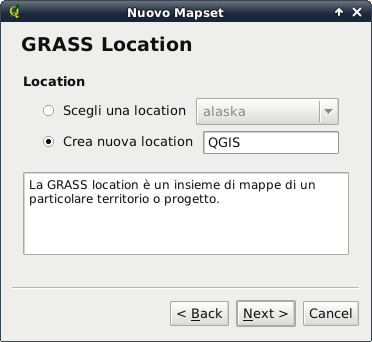
\includegraphics[clip=true, width=10cm]{create_grass_location}
\end{center}  
\end{figure}

\begin{enumerate}
  %\item Start QGIS and make sure the GRASS plugin is loaded
  \item D\'emarrez QGIS et assurez vous que l'extension GRASS est charg\'ee.
  %\item Visualize the \filename{alaska.shp} Shapefile (see Section \ref{sec:load_shapefile}) from the QGIS alaska dataset~\ref{label_sampledata}.
  \item Affichez le shapefile \filename{alaska.shp} (voir Section \ref{sec:load_shapefile}) du jeu de donn\'ees QGIS alaska ~\ref{label_sampledata}.
  %\item In the GRASS toolbar, click on the \toolbtntwo{grass_new_mapset}{Open mapset} icon to bring up the \filename{MAPSET} wizard.
  \item Dans la barre d'outils GRASS, cliquez sur \toolbtntwo{grass_new_mapset}{Nouveau jeu de donn\'ees} pour ouvrir l'assistant \filename{Jeux de donn\'ees}.
  %\item Select an existing GRASS database (GISDBASE) folder \filename{grassdata} or create one for the new \filename{LOCATION} using a file manager on your computer. Then click \button{Next}. 
  \item S\'electionnez un r\'epertoire existant de base de donn\'ees GRASS (Base de donn\'ees) \filename {grassdata} ou cr\'eez en un pour le nouveau \filename{SECTEUR} avec le gestionnaire de fichiers de votre ordinateur. Cliquez le bouton \button{Suivant}.
  %\item We can use this wizard to create a new \filename{MAPSET} within an existing \filename{LOCATION} (see Section~\ref{sec:add_mapset}) or to create a new \filename{LOCATION} altogether. Click on the radio button \radiobuttonon{Create new location} (see Figure \ref{fig:create_grass_location}).
  \item Nous pouvons utiliser cet assistant \`a la fois pour cr\'eer un nouveau \filename{Jeu de donn\'ees} dans un \filename{SECTEUR} existant (voir Section~\ref{sec:add_mapset}) et pour cr\'eer un nouveau \filename{SECTEUR}. Cliquez sur le bouton radio \radiobuttonon{Cr\'eez un nouveau secteur} (voir Figure \ref{fig:create_grass_location}).
  %\item Enter a name for the \filename{LOCATION} - we used alaska and click 
  \item Entrez un nom pour le \filename{SECTEUR} - nous utilisons alaska et cliquez sur le bouton \button{Suivant} 
  %\button{Next} 
  %\item Define the projection by clicking on the radio button \radiobuttonon{Projection} to enable the projection list 
  \item D\'efinissez la projection en cliquant sur le bouton radio \radiobuttonon{Projection} pour activer la liste des projections
  %\item We are using Albers Equal Area Alaska (feet) projection. Since we happen to know that it is represented by the EPSG ID 2964, we enter it in
  %the search box. (Note: If you want to repeat this process for another  \filename{LOCATION} and projection and haven't memorized the EPSG ID, 
  %click on the \toolbtntwo{mIconProjectionEnabled}{projector} icon in the lower right-hand  corner of the status bar (see Section \ref{label_projstart})).
  \item Nous utilisons la projection Albers Equal Area Alaska (pieds).\'Etant donn\'e que nous savons qu'elle correspond au code EPSG 2964, nous le saisissons dans le champ de recherche. (Note : Si vous souhaitez reproduire la manipulation pour un autre \filename{SECTEUR} et une autre projection et que vous ne connaissez pas le code EPSG, cliquez sur \toolbtntwo{mIconProjectionEnabled}{Statut de la projection} dans le coin inf\'erieur droit de la barre d'\'etat (voir Section \ref{label_projstart})).
  %\item Click \button{Find} to select the projection
  \item Cliquez sur \button{Trouver} pour s\'electionner la projection
  %\item Click \button{Next} 
  \item Cliquer sur \button{Suivant} 
  %\item To define the default region, we have to enter the \filename{LOCATION} bounds in north, south, east, and west direction. Here we simply click on the button \button{Set current QGIS extent}, to apply the extend of the loaded layer \filename{alaska.shp} as the GRASS default region extend.
  \item Pour d\'efinir la r\'egion par d\'efaut, nous devons saisir les limites Nord, Sud , Est et Ouest du \filename{SECTEUR}. Ici il suffit de cliquer sur le bouton \button{Fixer l'emprise courante de QGIS}, pour appliquer l'emprise du shapefile \filename{alaska.shp} d\'ej\`a charg\'e comme emprise par d\'efaut.
  %\item Click \button{Next} 
  \item Cliquer sur \button{Suivant} 
  %\item We also need to define a \filename{MAPSET} within our new \filename{LOCATION}. You can name it whatever you like - we used demo.\footnote{When creating a new \filename{LOCATION}, GRASS automatically creates a special \filename{MAPSET} called \filename{PERMANENT} designed to store the core data for the project, its default spatial extend and coordinate system definitions (Neteler \& Mitasova 2008  \cite{neteler_mitasova08}).}
  \item Nous avons aussi besoin de d\'efinir un \filename{Jeu de donn\'ees} dans notre nouveau \filename{SECTEUR}. Vous pouvez l'appeler comme vous le souhaitez - nous utiliserons demo. \footnote{Quand nous cr\'eons un nouveau \filename{SECTEUR}, GRASS cr\'e\'e automatiquement un \filename{Jeu de donn\'ees} sp\'ecial appel\'e \filename{PERMANENT} con\c{c}u pour stocker les donn\'ees essentiels du projet, l'extension spatiale par d\'efaut et la d\'efinition du syst\`eme de coordonn\'ees (Neteler \& Mitasova 2008  \cite{neteler_mitasova08}).}
  %\item Check out the summary to make sure it's correct and click \button{Finish} 
  \item V\'erifiez le r\'esum\'e pour vous assurez que tout est correct et cliquez sur \button{Terminer} 
  %\item The new \filename{LOCATION alaska} and two \filename{MAPSETs demo} and \filename{PERMANENT} are created. The currently opened working set is \filename{MAPSET demo}, as you defined.
  \item Le nouveau \filename{SECTEUR alaska} et les deux \filename{Jeux de donn\'ees demo} et \filename{PERMANENT} sont cr\'e\'es. Actuellement, le jeu de donn\'ees courant est le \filename{Jeux de donn\'ees demo}, tel que vous l'avez d\'efini.
  %\item Notice that some of the tools in the GRASS toolbar that were disabled are now enabled.
  \item Notez que certains outils qui n'\'etaient pas accessibles le sont maintenant.
\end{enumerate}

%If that seemed like a lot of steps, it's really not all that bad and a very quick way to create a \filename{LOCATION}. The \filename{LOCATION alaska} is 
%now ready for data import (see Section \ref{sec:import_loc_data}).You can also use the already existing vector and raster data in the sample 
%GRASS \filename{LOCATION alaska} included in the QGIS alaska dataset \ref{label_sampledata} and move on to Section \ref{label_vectmodel}.

Si cela semble faire beaucoup d'\'etapes, mais c'est en fait un moyen simple et rapide de cr\'eer un \filename{SECTEUR}. Le \filename{SECTEUR alaska} est maintenant pr\^et pour l'importation de donn\'ees (voir Section \ref{sec:import_loc_data}). Vous pouvez \'egalement utiliser des donn\'ees raster ou vecteur existantes dans le \filename{SECTEUR alaska} inclues dans le jeu de donn\'ees QGIS alaska \ref{label_sampledata} et continuez dans la section \ref{label_vectmodel}.

%\subsubsection{Adding a new MAPSET}\label{sec:add_mapset}
\subsubsection{Ajouter un nouveau Jeu de donn\'ees}\label{sec:add_mapset}

%A user has only write access to a GRASS \filename{MAPSET} he created. This means, besides access to his own \filename{MAPSET}, each user can also read 
%maps in other user's \filename{MAPSETs}, but he can modify or remove only the maps in his own \filename{MAPSET}. All \filename{MAPSETs} include a 
%\filename{WIND} file that stores the current boundary coordinate values and the currently selected raster resolution (Neteler \& Mitasova 2008 \cite{neteler_mitasova08}, see Section \ref{sec:grass_region}). 

Un utilisateur a seulement des droits d'\'ecriture sur le \filename{Jeu de donn\'ees} GRASS qu'il a cr\'e\'e. Cela veut dire qu'au del\`a de l'acc\`es \`a son propre \filename{Jeu de donn\'ees} GRASS, chaque utilisateur peut aussi lire les donn\'ees dans les autres \filename{Jeux de donn\'ees}, mais il ne peut modifier et supprimer que les donn\'ees que dans son propre \filename{Jeu de donn\'ees}. Tous les \filename{Jeux de donn\'ees} incluent un fichier \filename{WIND} qui stocke l'extension et la r\'esolution raster courante (Neteler \& Mitasova 2008 \cite{neteler_mitasova08}, voir Section \ref{sec:grass_region}). 


\begin{enumerate}
  %\item Start QGIS and make sure the GRASS plugin is loaded
  \item D\'emarrer QGIS et assurez vous que l'extension GRASS est charg\'ee
  %\item In the GRASS toolbar, click on the \toolbtntwo{grass_new_mapset}{New mapset} icon to bring up the \filename{MAPSET} wizard.
  \item Dans la barre d'outils GRASS, cliquez sur \toolbtntwo{grass_new_mapset}{Nouveau jeu de donn\'ees} pour ouvrir l'assistant \filename{Jeux de donn\'ees}.
  %\item Select the GRASS database (GISDBASE) folder \filename{grassdata}  with the \filename{LOCATION alaska}, where we want to add a further \filename{MAPSET}, called test.
  \item S\'electionnez le r\'epertoire \filename{grassdata} de la base de donn\'ees GRASS (Base de donn\'ees) qui contient d\'ej\`a le \filename{SECTEUR alaska} et o\`u nous voulons ajouter un autre \filename{SECTEUR} appel\'e test.
  %\item Click \button{Next}. 
  \item Cliquez sur \button{Suivant}. 
  %\item We can use this wizard to create a new \filename{MAPSET} within an existing \filename{LOCATION} or to create a new \filename{LOCATION} altogether. Click on the radio button \radiobuttonon{Select location} (see Figure \ref{fig:create_grass_location}) and click \button{Next}.
  \item Nous pouvons utiliser cet assistant \`a la fois pour cr\'eer un nouveau \filename{Jeu de donn\'ees} dans le \filename{SECTEUR} existant et pour cr\'eer un nouveau \filename{SECTEUR}. Cliquez sur le bouton radio \radiobuttonon{S\'electionnez le Secteur} (voir Figure \ref{fig:create_grass_location}) et cliquez sur \button{Suivant}.
  %\item Enter the name \filename{text} for the new \filename{MAPSET}. Below in the wizard you see a list of existing \filename{MAPSETs} and its owners.
  \item Entrez le \filename{text} du nom pour le nouveau \filename{Jeu de donn\'ees}. En dessous, dans l'assistant, vous pouvez voir une liste des \filename{Jeux de donn\'ees} et de leurs propri\'etaires.
  %\item Click \button{Next}, check out the summary to make sure it's all correct and click \button{Finish}
  \item Cliquez sur \button{Suivant}, v\'erifiez le r\'esum\'e pour vous assurer qu'il est correct et cliquez sur \button{Terminer} 
\end{enumerate}

%\subsection{Importing data into a GRASS LOCATION}\label{sec:import_loc_data}
\subsection{Importer des donn\'ees dans un SECTEUR GRASS}\label{sec:import_loc_data}
%This Section gives an example how to import raster and vector data into the \filename{alaska} GRASS \filename{LOCATION} provided by the QGIS alaska dataset.
%Therefore we use a landcover raster map \filename{landcover.img} and a vector GML File \filename{lakes.gml} from the QGIS alaska dataset \ref{label_sampledata}.
Cette section donne un exemple d'importation de donn\'ees raster et vecteur dans le \filename{SECTEUR} GRASS \filename{alaska} fournit dans le jeu de donn\'ees QGIS alaska. Nous utiliserons une couche raster d'occupation du sol \filename{landcover.img} et une couche vecteur au format GML \filename{lakes.gml}, toutes deux pr\'esentes dans le jeu de donn\'ees alaska.
\begin{enumerate}
  %\item Start QGIS and make sure the GRASS plugin is loaded.
  \item D\'emarrer QGIS et assurez vous que l'extension GRASS est charg\'ee.
  %\item In the GRASS toolbar, click the \toolbtntwo{grass_open_mapset}{Open MAPSET} icon to bring up the \filename{MAPSET} wizard.
  \item Dans la barre d'outil GRASS, cliquez sur \toolbtntwo{grass_open_mapset}{Ouvrir un jeu de donn\'ees} pour ouvrir l'assistant \filename{Jeu de donn\'ees}.
  %\item Select as GRASS database the folder \filename{grassdata} in the QGIS alaska dataset, as \filename{LOCATION alaska}, as \filename{MAPSET} 
  %\filename{demo} and click \button{OK}.
  \item S\'electionnez comme base de donn\'ees GRASS le r\'epertoire \filename{grassdata} dans le jeu de donn\'ees QGIS alaska, comme \filename{SECTEUR alaska}, comme as \filename{Jeu de donn\'ee} \filename{demo} et cliquez sur \button{OK}.
  %\item Now click the \toolbtntwo{grass_tools}{Open GRASS tools} icon. The GRASS Toolbox (see Section \ref{subsec:grass_toolbox}) dialog appears.
  \item Maintenant cliquez sur \toolbtntwo{grass_tools}{Ouvrir les outils GRASS}. La bo\^ite \`a outils GRASS (voir Section \ref{subsec:grass_toolbox}) s'ouvre.
  %\item To import the raster map \filename{landcover.img}, click the module \filename{r.in.gdal} in the \tab{Modules Tree} tab. This GRASS module allows to import GDAL supported raster files into a GRASS \filename{LOCATION}. The module dialog for \filename{r.in.gdal} appears.
  \item  Pour importer la couche raster \filename{landcover.img}, cliquez sur le module \filename{r.in.gdal} dans l'onglet \tab{Arborescence des modules}. Ce module GRASS vous permet d'importer les fichiers raster support\'es par la librairie GDAL dans un \filename{SECTEUR} GRASS. La bo\^ite de dialogue  \filename{r.in.gdal} appara\^it.
  %\item Browse to the folder \filename{raster} in the QGIS alaska dataset and select the file \filename{landcover.img}.
  \item Naviguer jusqu'au r\'epertoire \filename{raster} dans le jeu de donn\'ees QGIS alaska et s\'electionnez le fichier \filename{landcover.img}.
  %\item As raster output name define \filename{landcover\_grass} and click \button{Run}. In the \tab{Output} tab you see the currently running GRASS command \filename{r.in.gdal -o input=/path/to/landcover.img output=landcover\_grass}.
  \item D\'efinissez \filename{landcover\_grass} comme nom de sortie et cliquez sur \button{Lancer}. Dans l'onglet \tab{Rendu}, vous voyez la commande GRASS en cours \filename{r.in.gdal -o input=/path/to/landcover.img output=landcover\_grass}.
  %\item When it says \textbf{Succesfully finished} click \button{View output}. 
  \item Lorsque \textbf{Termin\'e avec succ\`es} s'affiche cliquez sur \button{Vue}. 
  %The \filename{landcover\_grass} raster layer is now imported into GRASS and will be visualized in the QGIS canvas.
  La couche raster \filename{landcover\_grass} est maintenant import\'ee dans GRASS et pourra \^etre affich\'ee dans QGIS.
  
  %\item To import the vector GML file \filename{lakes.gml}, click the module \filename{v.in.ogr} in the \tab{Modules Tree} tab. This GRASS module allows to import OGR supported vector files into a GRASS \filename{LOCATION}. The module dialog for \filename{v.in.ogr} appears.
  \item Pour importer le fichier GML \filename{lakes.gml}, cliquez sur le module \filename{v.in.ogr} dans l'onglet \tab{Arborescence des modules}.La bo\^ite de dialogue  \filename{v.in.ogr} appara\^it.
  %\item Browse to the folder \filename{gml} in the QGIS alaska dataset and select the file \filename{lakes.gml} as OGR file.
  \item Naviguer jusqu'au r\'epertoire \filename{gml} dans le jeu de donn\'ees QGIS alaska et s\'electionnez le fichier \filename{lakes.gml}.
  %\item As vector output name define \filename{lakes\_grass} and click \button{Run}. You don't have to care about the other options in this   example. In the \tab{Output} tab you see the currently running GRASS command \filename{v.in.ogr -o dsn=/path/to/lakes.gml output=lakes\_grass}.
  \item D\'efinissez \filename{lakes\_grass} comme nom de sortie et cliquez sur \button{Lancer}. Vous n'avez pas besoin des autres options dans cet exemple.
  %\item When it says \textbf{Succesfully finished} click \button{View output}. 
  \item Lorsque \textbf{Termin\'e avec succ\`es} s'affiche cliquez sur \button{Vue}. 
  %The \filename{lakes\_grass} vector layer is now imported into GRASS and will be visualized in the QGIS canvas. 
  Le fichier \filename{lakes\_grass} est maintenant import\'e dans GRASS et pourra \^etre affich\'e dans QGIS.
\end{enumerate}


%\subsection{The GRASS vector data model}\label{label_vectmodel}\index{GRASS!vector datamodel}
\subsection{Le mod\`ele vecteur de GRASS}\label{label_vectmodel}\index{GRASS!mod\`ele vecteur}
%It is important to understand the GRASS vector data model prior to digitizing.\index{GRASS!digitizing} In general, GRASS uses a topological vector model.\index{GRASS!topology} This means that areas are not represented as closed polygons, but by one or more boundaries. A boundary between two adjacent areas is digitized only once, and it is shared by both areas. Boundaries must be connected without gaps. An area is identified (labeled) by the centroid of the area.
Il est important de comprendre le mod\`ele vecteur de GRASS avant de faire de la num\'erisation.\index{GRASS!num\'erisation} En g\'en\'eral, GRASS utilise un mod\`ele vecteur topologique.\index{GRASS!topologie} Cela veut dire que les surfaces ne sont pas repr\'esent\'ees par des polygones ferm\'es mais par une ou plusieurs limites. Une limite entre des polygones adjacents n'est num\'eris\'ee qu'une seule fois et est partag\'ee par les deux surfaces. Les limites doivent \^etre connect\'ees sans trous. Une surface est identifi\'ee (libell\'ee) via le centroide de la surface.

%Besides boundaries and centroids, a vector map can also contain points and lines. All these geometry elements can be mixed in one vector and will be represented in different so called 'layers' inside one GRASS vector map. So in GRASS a layer is not a vector or raster map but a level inside a vector layer. This is important to distinguish carefully.
	
Outre les limites et centro"ides, une couche vecteur peut \'egalement contenir des points et des lignes. Tous ces \'el\'ements de g\'eom\'etrie peuvent \^etre m\'elang\'es dans une couche vecteur et seront repr\'esent\'es dans diff\'erentes «sous-couches» dans une carte vectorielle GRASS. Ainsi, une couche GRASS n'est pas un vecteur ou un raster, mais un niveau \`a l'int\'erieur d'une couche vecteur. Il est important de bien distinguer ceci.

%\footnote{Although it is possible to mix geometry elements, it is unusual and even in GRASS only used in special cases such as vector network analysis. Normally you should
%prefere to store different geometry elements in different layers.}
\footnote{M\^eme s'il est possible de m\'elanger des \'el\'ements de g\'eom\'etries diff\'erentes, c'est inhabituel et m\^eme dans GRASS, on l'utilise dans des cas particuliers tel que l'analyse de r\'eseau. Normalement, vous devriez stocker des \'el\'ements de g\'eom\'etries diff\'erentes dans des couches diff\'erentes}

%It is possible to store more 'layers' in one vector dataset. For example, fields, forests and lakes can be stored in one vector. Adjacent forest and lake can share the same boundary, but they have separate attribute tables. It is also possible to attach attributes to boundaries. For example, the boundary between lake and forest is a road, so it can have a different attribute table.
Il est possible de stocker plusieurs sous-couches dans une couche vecteur. Par exemple, des champs, de la for\^et et des lacs peuvent \^etre stock\'es dans une couche vecteur. Les for\^ets et les lacs adjacents partagent les m\^emes limites, mais ils auront des tables attributaires diff\'erentes. Il est aussi possible de faire correspondre une table attributaires aux limites. Par exemple, la limite entre un lac et une for\^et peut \^etre une route qui peut avoir une table attributaire diff\'erente.

%The 'layer' of the feature is defined by 'layer' inside GRASS. 'Layer' is the number which defines if there are more than one layer inside the dataset, e.g. if the geometry is forest or lake. For now, it can be only a number, in the future GRASS will also support names as fields in the user interface.
La 'sous-couche' est d\'efinie dans GRASS par un chiffre. Ce chiffre d\'efinit s'il y a plusieurs sous-couches \`a l'int\'erieur d'une couche vecteur. Par exemple, il d\'efinit s'il s'agit de lac ou de for\^et. Pour l'instant, il s'agit d'un nombre mais dans des versions futures GRASS pourra utiliser des noms pour les sous-couches dans l'interface utilisateur.

%Attributes can be stored inside the GRASS \filename{LOCATION} as DBase or SQLITE3 or in external database tables, for example PostgreSQL, MySQL, Oracle, etc.\index{GRASS!attribute storage}
Les donn\'ees attributaires peuvent \^etre stock\'ees dans le \filename{SECTEUR} au format DBase ou SQLIte3 ou dans des tables de bases de donn\'ees externes comme par exemple : PostgreSQL, MySQL, Oracle, etc.\index{GRASS!stockage des attributs}

%Attributes in database tables are linked to geometry elements using a 'category' value.\index{GRASS!attribute linkage} 'Category' (key, ID) is an
%integer attached to geometry primitives, and it is used as the link to one key column in the database table.
Les donn\'ees attributaires sont li\'ees \`a la g\'eom\'etrie par le biais d'un champ 'category'.\index{GRASS!liens des attributs} 'Category' (cl\'e, ID) est un entier attach\'e \`a la g\'eom\'etrie, et il est utilis\'e comme lien vers une colonne de cl\'e dans la table de base de donn\'ees.


%\begin{Tip}\caption{\textsc{Learning the GRASS Vector Model}}
\begin{Astuce}\caption{\textsc{Apprendre le mod\`ele vecteur de GRASS}}
\qgistip{
%The best way to learn the GRASS vector model and its capabilities is to download one of the many GRASS tutorials where the vector model is described
%more deeply. See \url{http://grass.osgeo.org/gdp/manuals.php} for more information, books and tutorials in several languages.
Le meilleur moyen d'apprendre le mod\`ele vecteur de GRASS et ses possibilit\'es est de t\'el\'echarger un des nombreux tutoriels GRASS o\`u le mod\`ele vecteur est d\'ecrit plus pr\'ecis\'ement. Voir \url{http://grass.osgeo.org/gdp/manuals.php} pour des informations compl\'ementaires, des livres et des tutoriels dans diff\'erentes langues.
}
\end{Astuce} 

%\subsection{Creating a new GRASS vector layer}\label{sec:creating_new_grass_vectors}\index{GRASS!Creating new vectors|see{editing!creating a new layer}}
\subsection{Cr\'eation d'une nouvelle couche vecteur GRASS}\label{sec:creating_new_grass_vectors}\index{GRASS!Cr\'eer de nouvelles couches vecteur|voir{\'editer!cr\'eer une nouvelle couche}}

%To create a new GRASS vector layer with the GRASS plugin click the \toolbtntwo{grass_new_vector_layer}{Create new GRASS vector} toolbar icon. 
%Enter a name in the text box and you can start digitizing point, line or polygone geometries, following the procedure described in Section \ref{grass_digitising}. 
Pour cr\'eer une nouvelle couche vecteur GRASS \`a l'aide de l'extension GRASS, cliquez sur \toolbtntwo{grass_new_vector_layer}{Cr\'eez une nouvelle couche vectorielle GRASS} dans la barre d'outils. Entrez le nom dans la bo\^ite de dialogue et vous pouvez commencer \`a digitaliser un point une ligne ou un polygone en suivant les instructions de la section \ref{grass_digitising}.
%In GRASS it is possible to organize all sort of geometry types (point, line and area) in one layer, because GRASS uses a topological vector model, so you don't need to select the geometry type when creating a new GRASS vector. This is different from Shapefile creation with QGIS, because Shapefiles use the Simple Feature vector model (see Section \ref{sec:create shape}).
Dans GRASS, il est possible de g\'erer plusieurs types de g\'eom\'etrie (point, ligne et surface) dans une seule couche d'information, car GRASS utilise un mod\`ele vecteur topologique. Vous n'avez donc pas besoin de s\'electionner un type de g\'eom\'etrie quand vous cr\'eez une couche vecteur GRASS. C'est diff\'erent de la cr\'eation de shapefile avec QGIS, car les shapefiles utilisent un mod\`ele vecteur d'entit\'e simple (Simple Feature vector model) (voir Section \ref{sec:create shape}).

%\begin{Tip}\caption{\textsc{Creating an attribute table for a new GRASS vector layer}}
\begin{Astuce}\caption{\textsc{Cr\'eation d'une table attributaire pour une nouvelle couche vecteur GRASS}}
\qgistip{
%If you want to assign attributes to your digitized geometry features, make sure to create an attribute table with columns before you start digitizing (see Figure \ref{fig:grass_digitizing_table}).
Si vous souhaitez renseigner les donn\'ees attributaires de vos entit\'es num\'eris\'ees, assurez-vous d'avoir cr\'e\'e une table attributaire avec des champs avant ce commencer votre num\'erisation (voir Figure \ref{fig:grass_digitizing_table}).
}
\end{Astuce} 

%\subsection{Digitizing and editing a GRASS vector layer}\index{GRASS!digitizing tools}\label{grass_digitising}
\subsection{Num\'erisation et \'edition de couche vecteur GRASS}\index{GRASS!outils de num\'erisation}\label{grass_digitising}

%The digitizing tools for GRASS vector layers are accessed using the \toolbtntwo{grass_edit}{Edit GRASS vector layer} icon on the toolbar. Make 
%sure you have loaded a GRASS vector and it is the selected layer in the legend before clicking on the edit tool. Figure \ref{fig:grass_digitizing_category} shows the GRASS edit dialog that is displayed when you click on the edit tool. The tools and settings are discussed in the following sections.
Les outils de num\'erisation pour les couches vecteurs de GRASS sont accessibles via \toolbtntwo{grass_edit}{\'Editer une couche vectorielle GRASS} dans la barre d'outils. Assurez-vous d'avoir ouvert une couche vectorielle GRASS ainsi que d'avoir s\'electionn\'e la sous-couche dans la l\'egende avant d'utiliser l'outil d'\'edition. La figure \ref{fig:grass_digitizing_category} montre la bo\^ite de dialogue GRASS qui s'affiche quand vous cliquez sur l'outil d'\'edition. Les outils et les param\`etres d'\'edition sont d\'etaill\'es dans les sections suivantes.

%\begin{Tip}\caption{\textsc{Digitizing polygones in GRASS}}
\begin{Astuce}\caption{\textsc{Num\'erisation de polygones dans GRASS}}
\qgistip{
%If you want to create a polygone in GRASS, you first digitize the boundary of the polygone, setting the mode to \usertext{No category}. Then you add a centroid (label point) into the closed boundary, setting the mode to \usertext{Next not used}. The reason is, that a topological vector model links attribute information of a polygon always to the centroid and not to the boundary.
Si vous voulez cr\'eer un polygone dans GRASS, vous devez num\'eriser premi\`erement les limites du polygone, en d\'efinissant mode sur \usertext{Pas de cat\'egorie}.Ensuite, vous ajoutez un centro"ide (emplacement de l'\'etiquette) dans le polygone ferm\'e, fixant le mode sur \usertext{Prochain non utilis\'e}. La raison en est, que le mod\`ele vectoriel topologique assure toujours le lien entre les informations d'attributs des polygones via le centro"ide et non via la limite.}
\end{Astuce} 

\minisec{Barre d'outils}\label{label_grasstoolbar}

%In Figure \ref{fig:grass_digitizing_toolbar} you see the GRASS digitizing toolbar icons provided by the GRASS plugin. Table \ref{tab:grass_tools}
%explains the available functionalities.
Sur la figure \ref{fig:grass_digitizing_toolbar} vous pouvez voir la barre d'outils d'\'edition GRASS de l'extension GRASS. Le tableau \ref{tab:grass_tools} r\'ecapitule les fonctions disponibles.

\begin{figure}[h]
   \begin{center}
%   \caption{GRASS Digitizing Toolbar \nixcaption}\label{fig:grass_digitizing_toolbar} 
   \caption{Barre d'outils d'\'edition GRASS \nixcaption}\label{fig:grass_digitizing_toolbar} 
   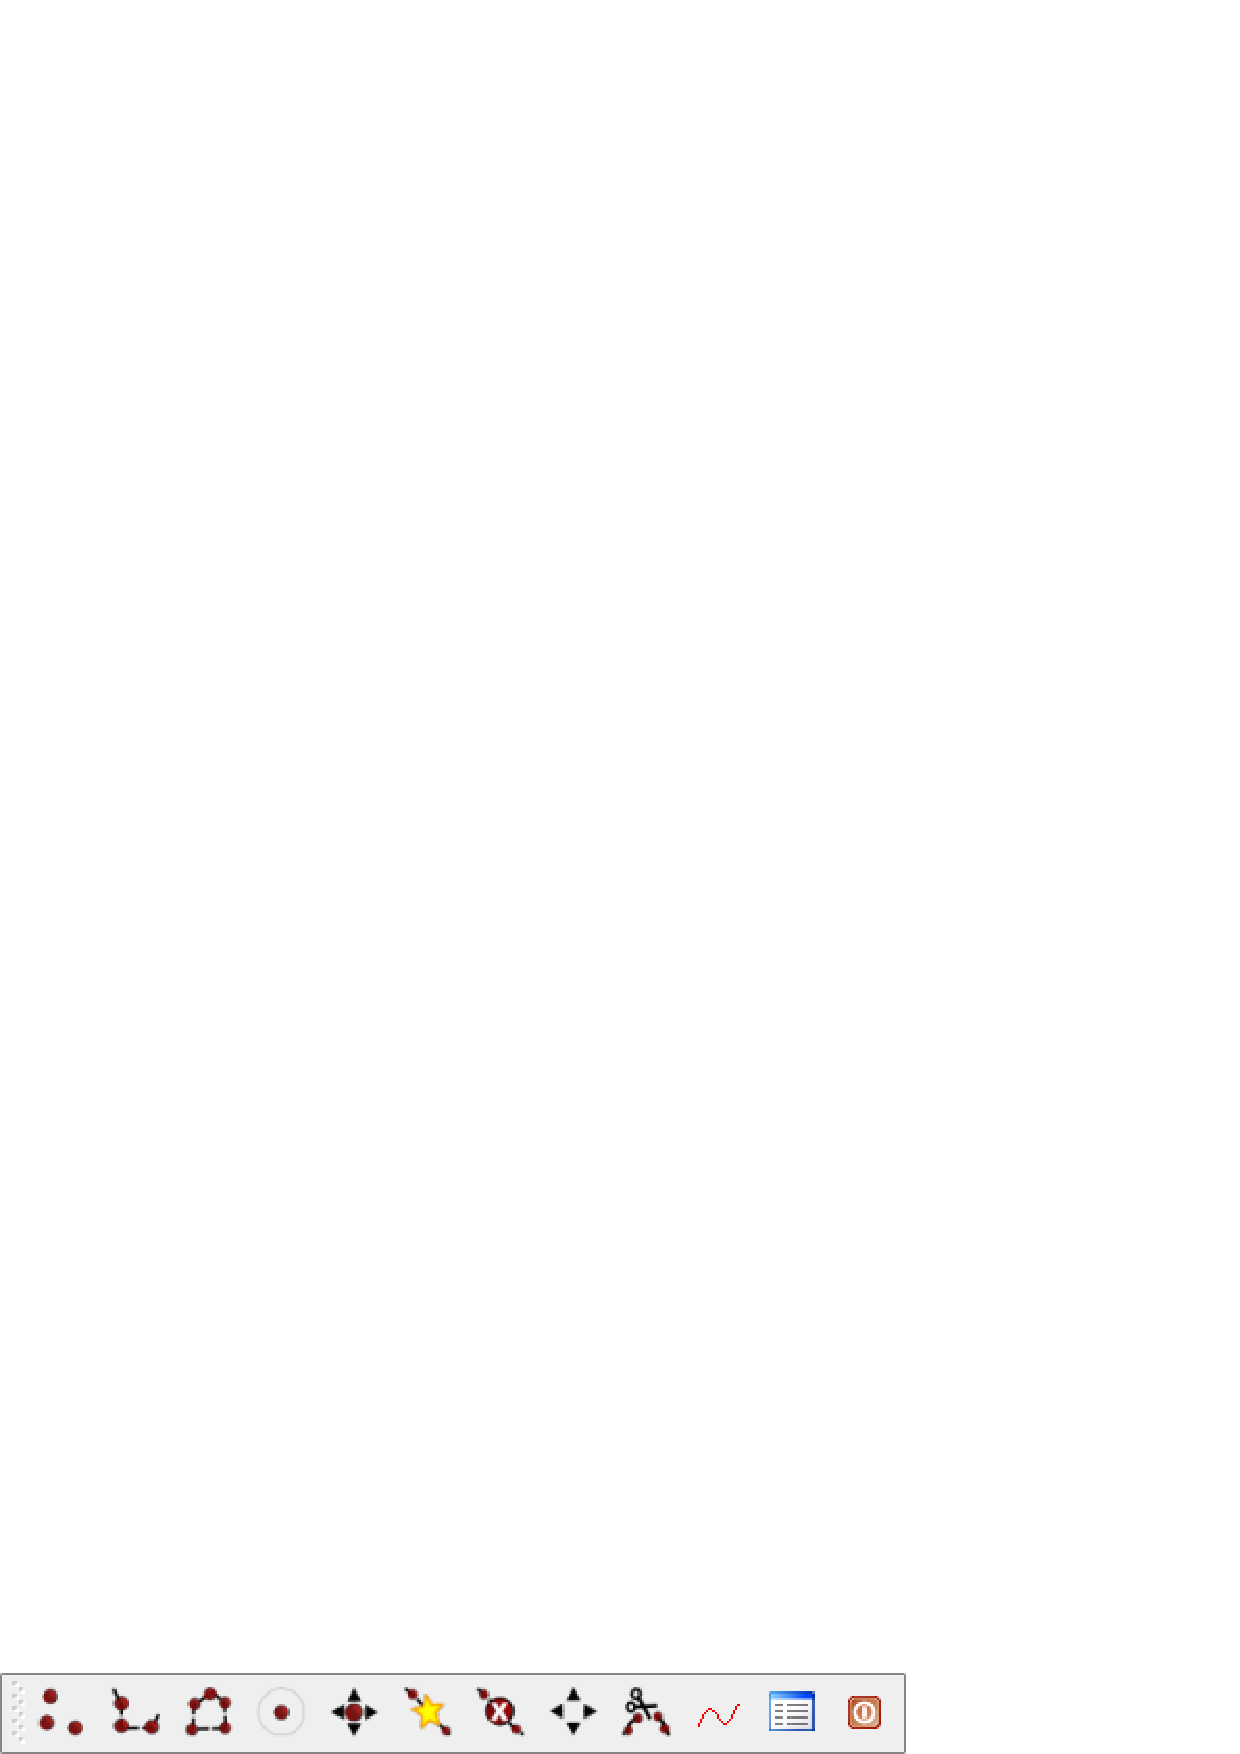
\includegraphics[clip=true,width=12cm]{grass_digitizing_toolbar}
\end{center}  
\end{figure}

%\begin{table}[h]\index{GRASS!digitizing tools}
\begin{table}[h]\index{GRASS!outils de num\'erisation}
\centering
%\caption{GRASS Digitizing Tools}\label{tab:grass_tools}\medskip
\caption{Outils de num\'erisation GRASS}\label{tab:grass_tools}\medskip
 \begin{tabular}{|l|l|p{5in}|}
%\hline \textbf{Icon} & \textbf{Tool} & \textbf{Purpose} \\
%\hline 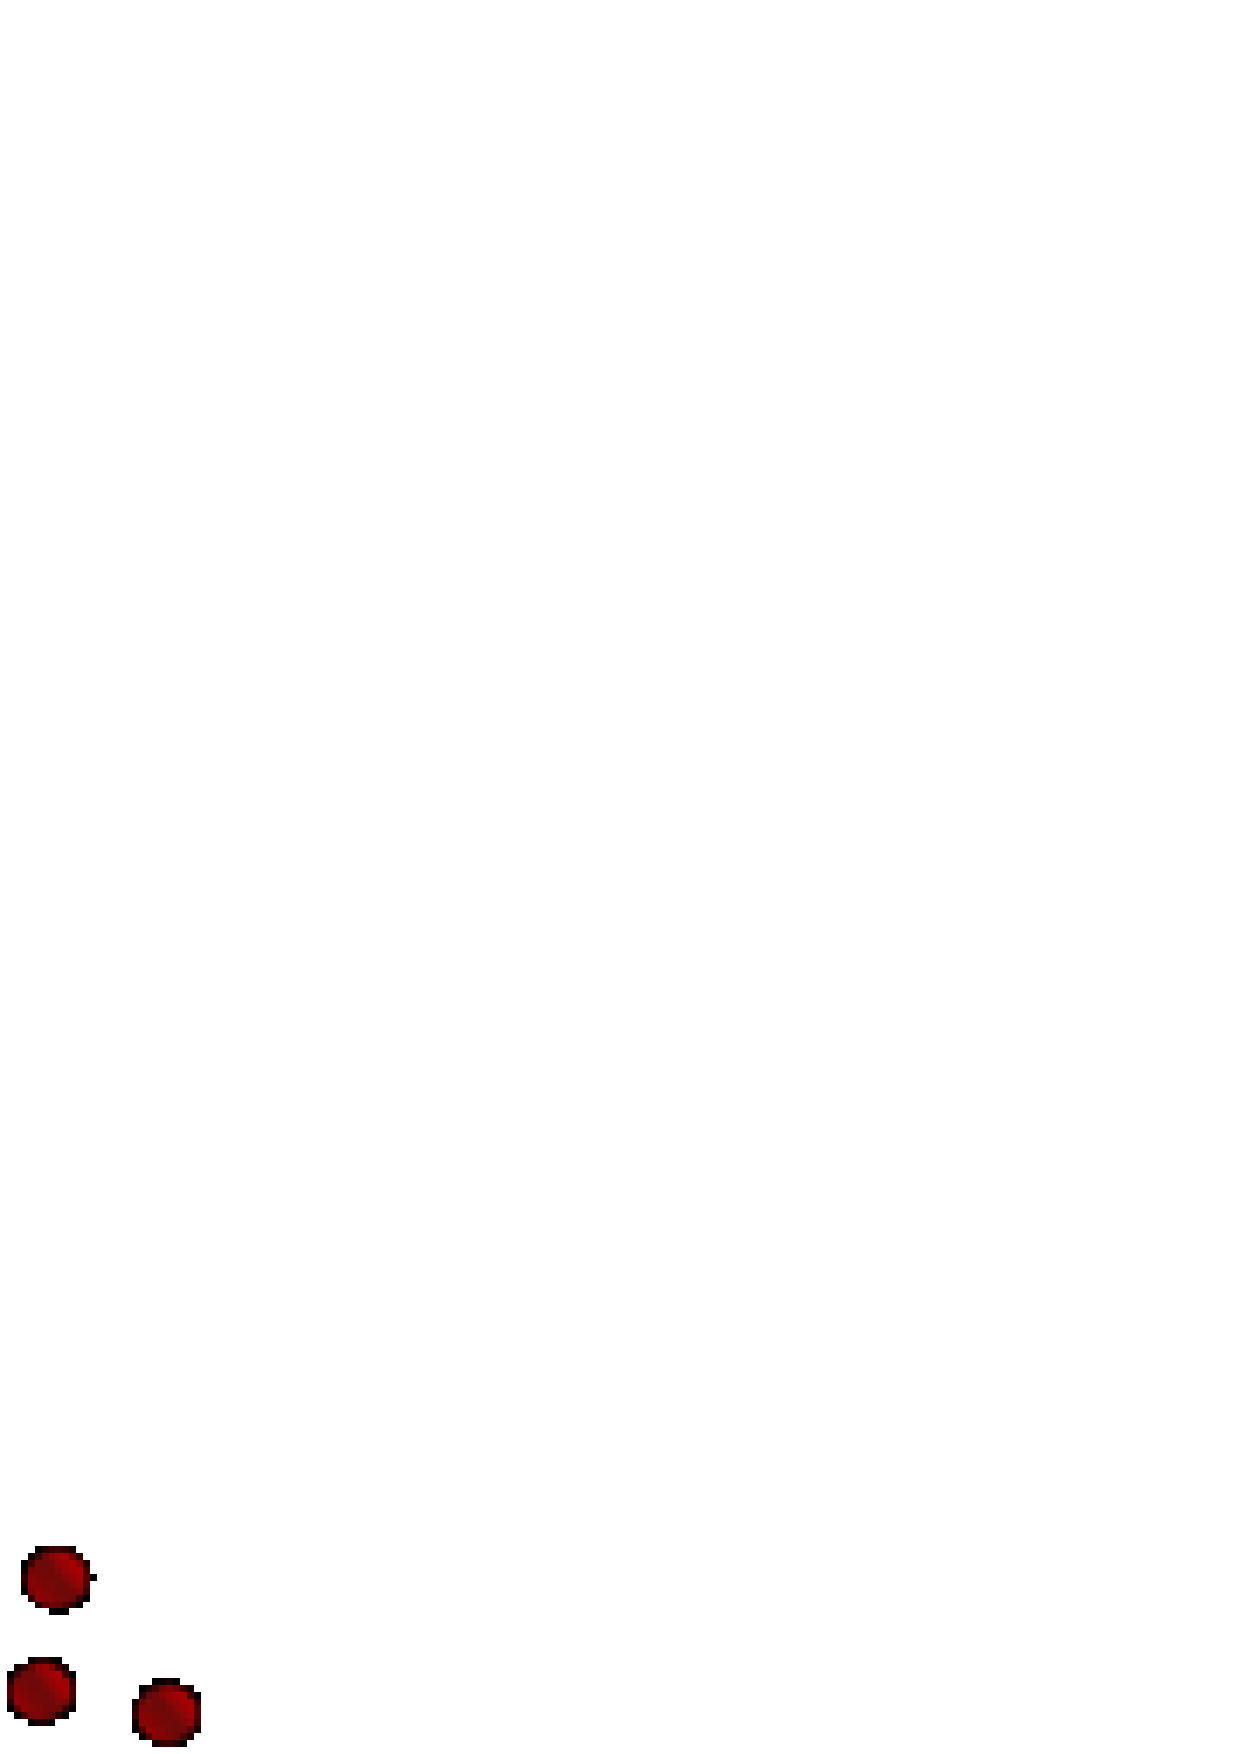
\includegraphics[width=0.7cm]{grass_new_point} & New Point & Digitize new point \\
%\hline 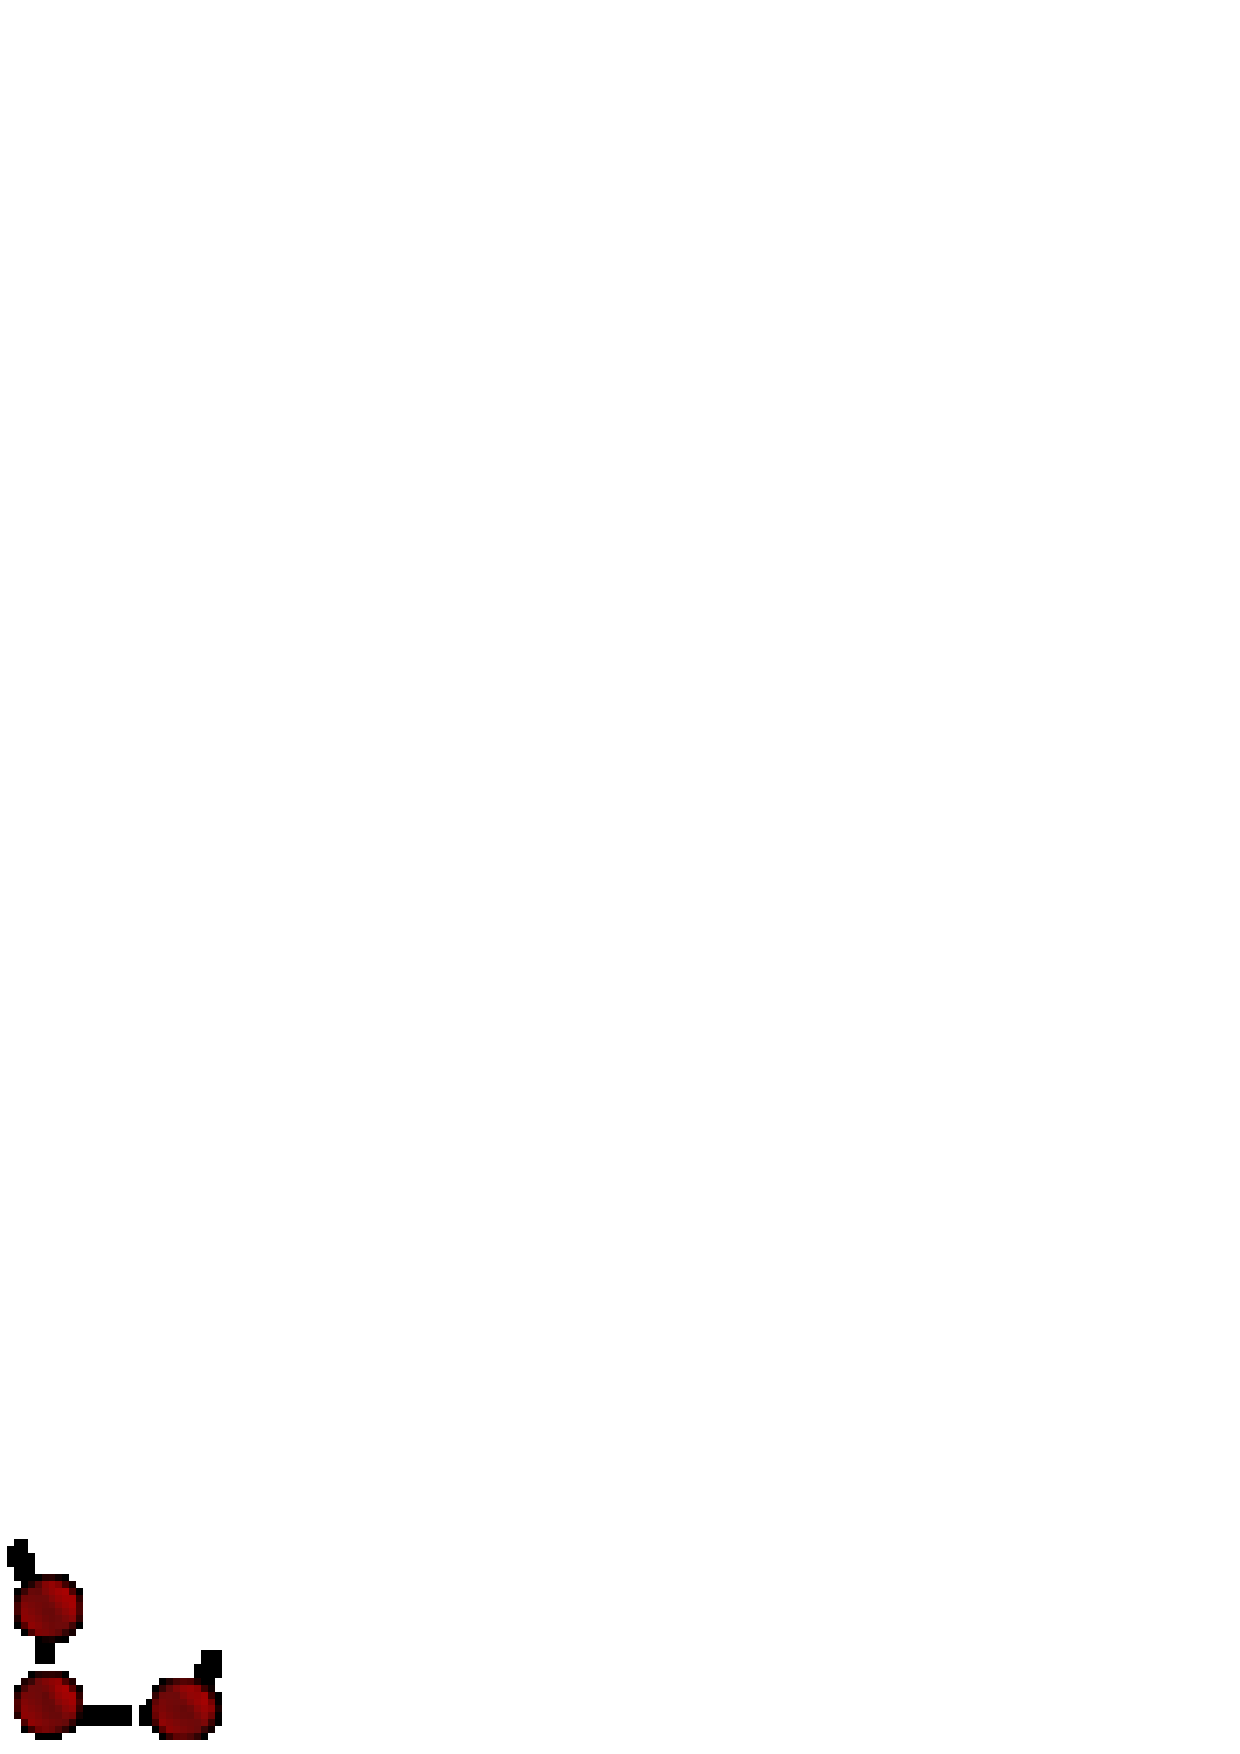
\includegraphics[width=0.7cm]{grass_new_line} & New Line & Digitize new line (finish by selecting new tool) \\
%\hline 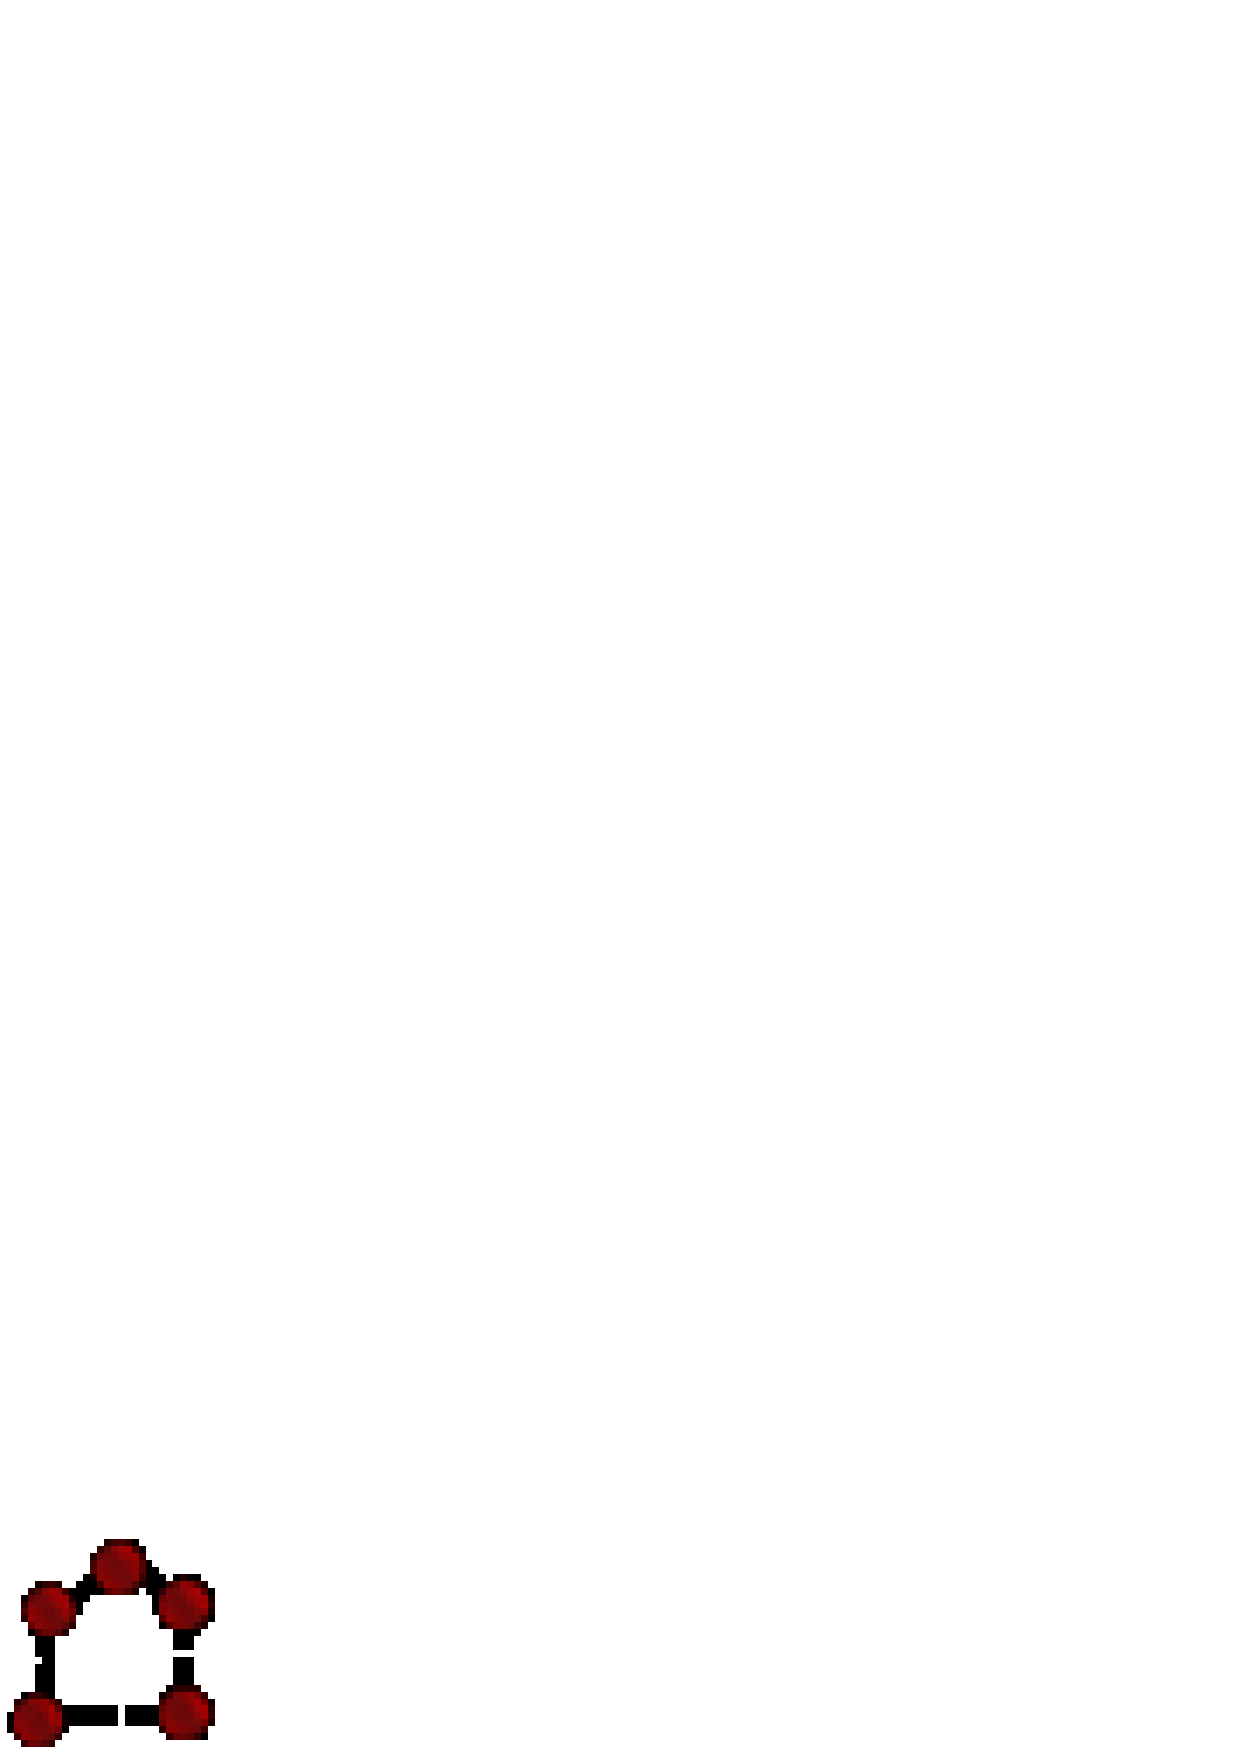
\includegraphics[width=0.7cm]{grass_new_boundary} & New Boundary & Digitize new boundary (finish by selecting new tool)\\
%\hline 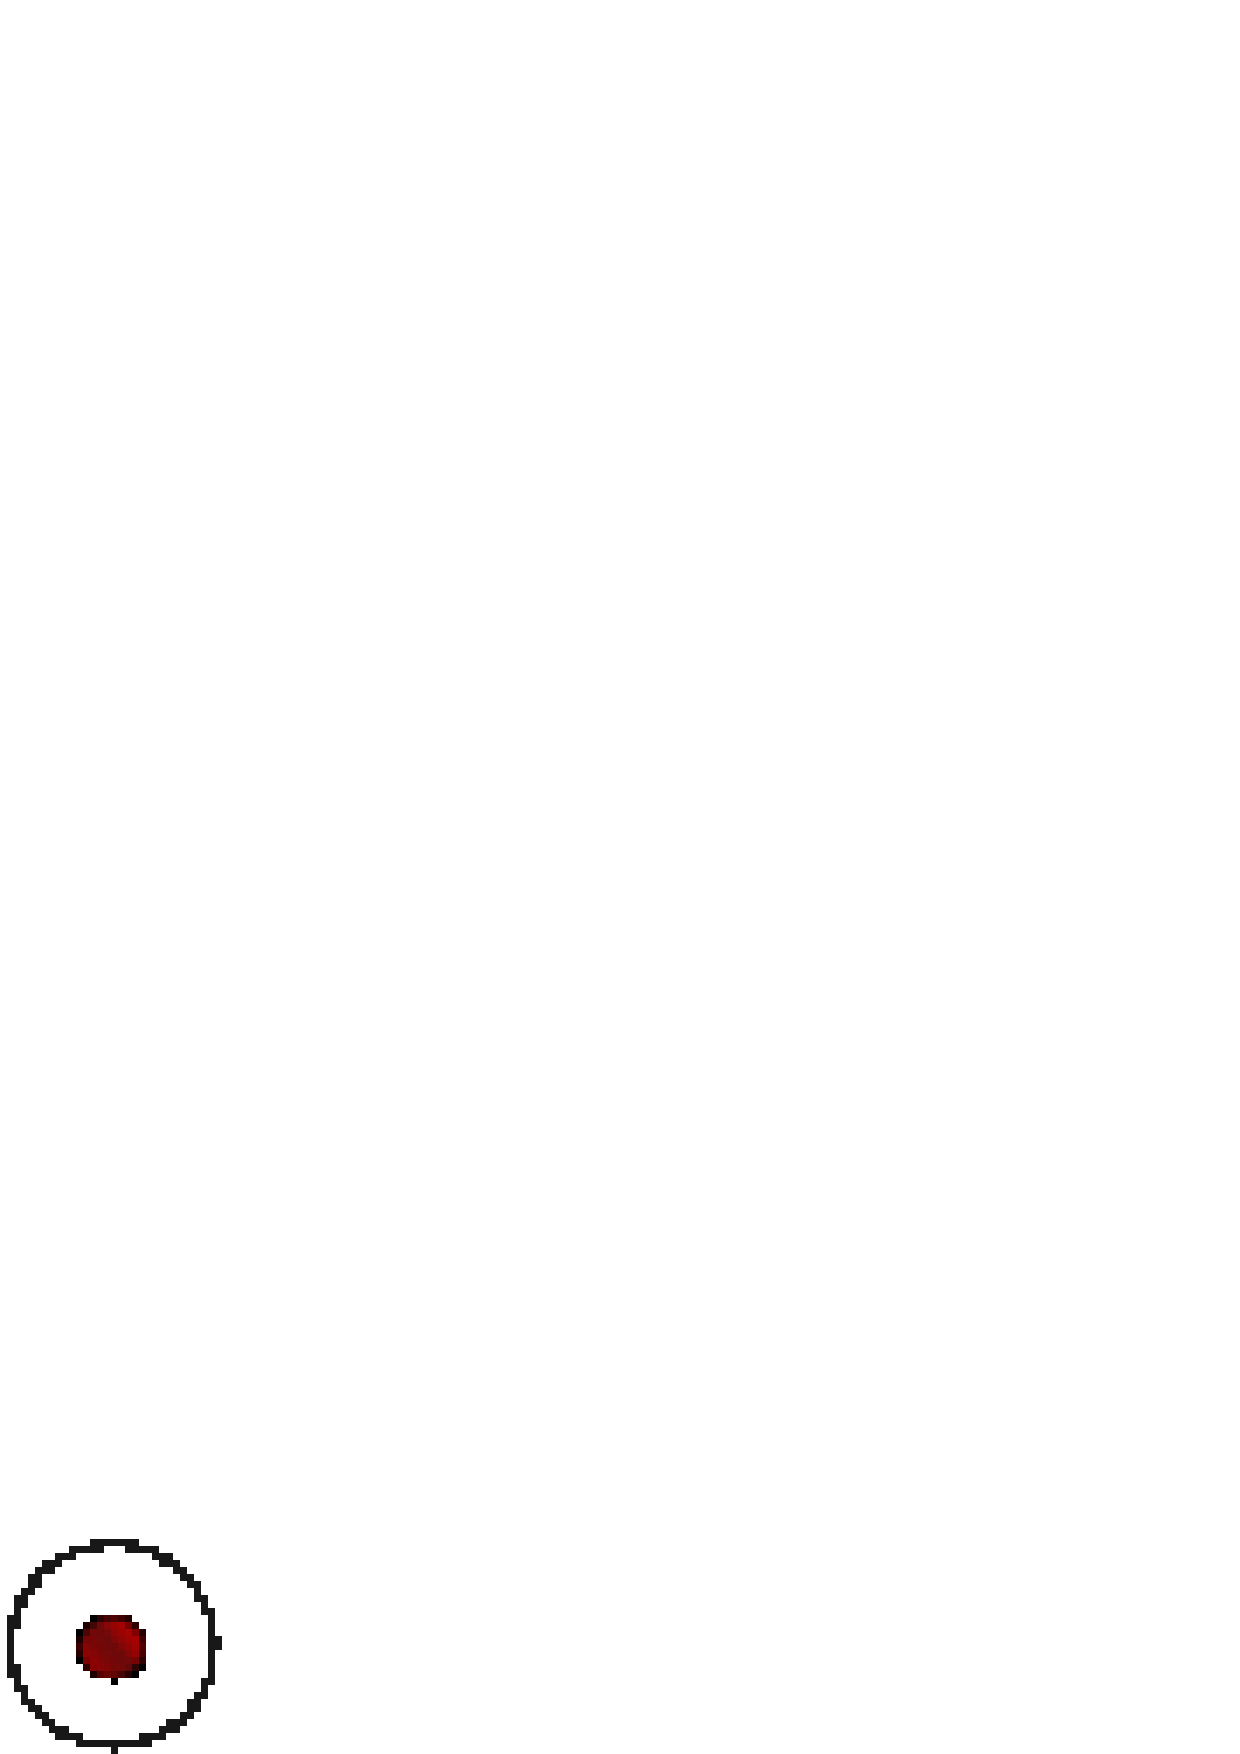
\includegraphics[width=0.7cm]{grass_new_centroid} & New Centroid & Digitize new centroid (label existing area)\\
%\hline 
\includegraphics[width=0.7cm]{grass_move_vertex} & Move vertex & Move one vertex of existing line or boundary and identify new position\\
%\hline 
\includegraphics[width=0.7cm]{grass_add_vertex} & Add vertex & Add a new vertex to existing line\\
%\hline 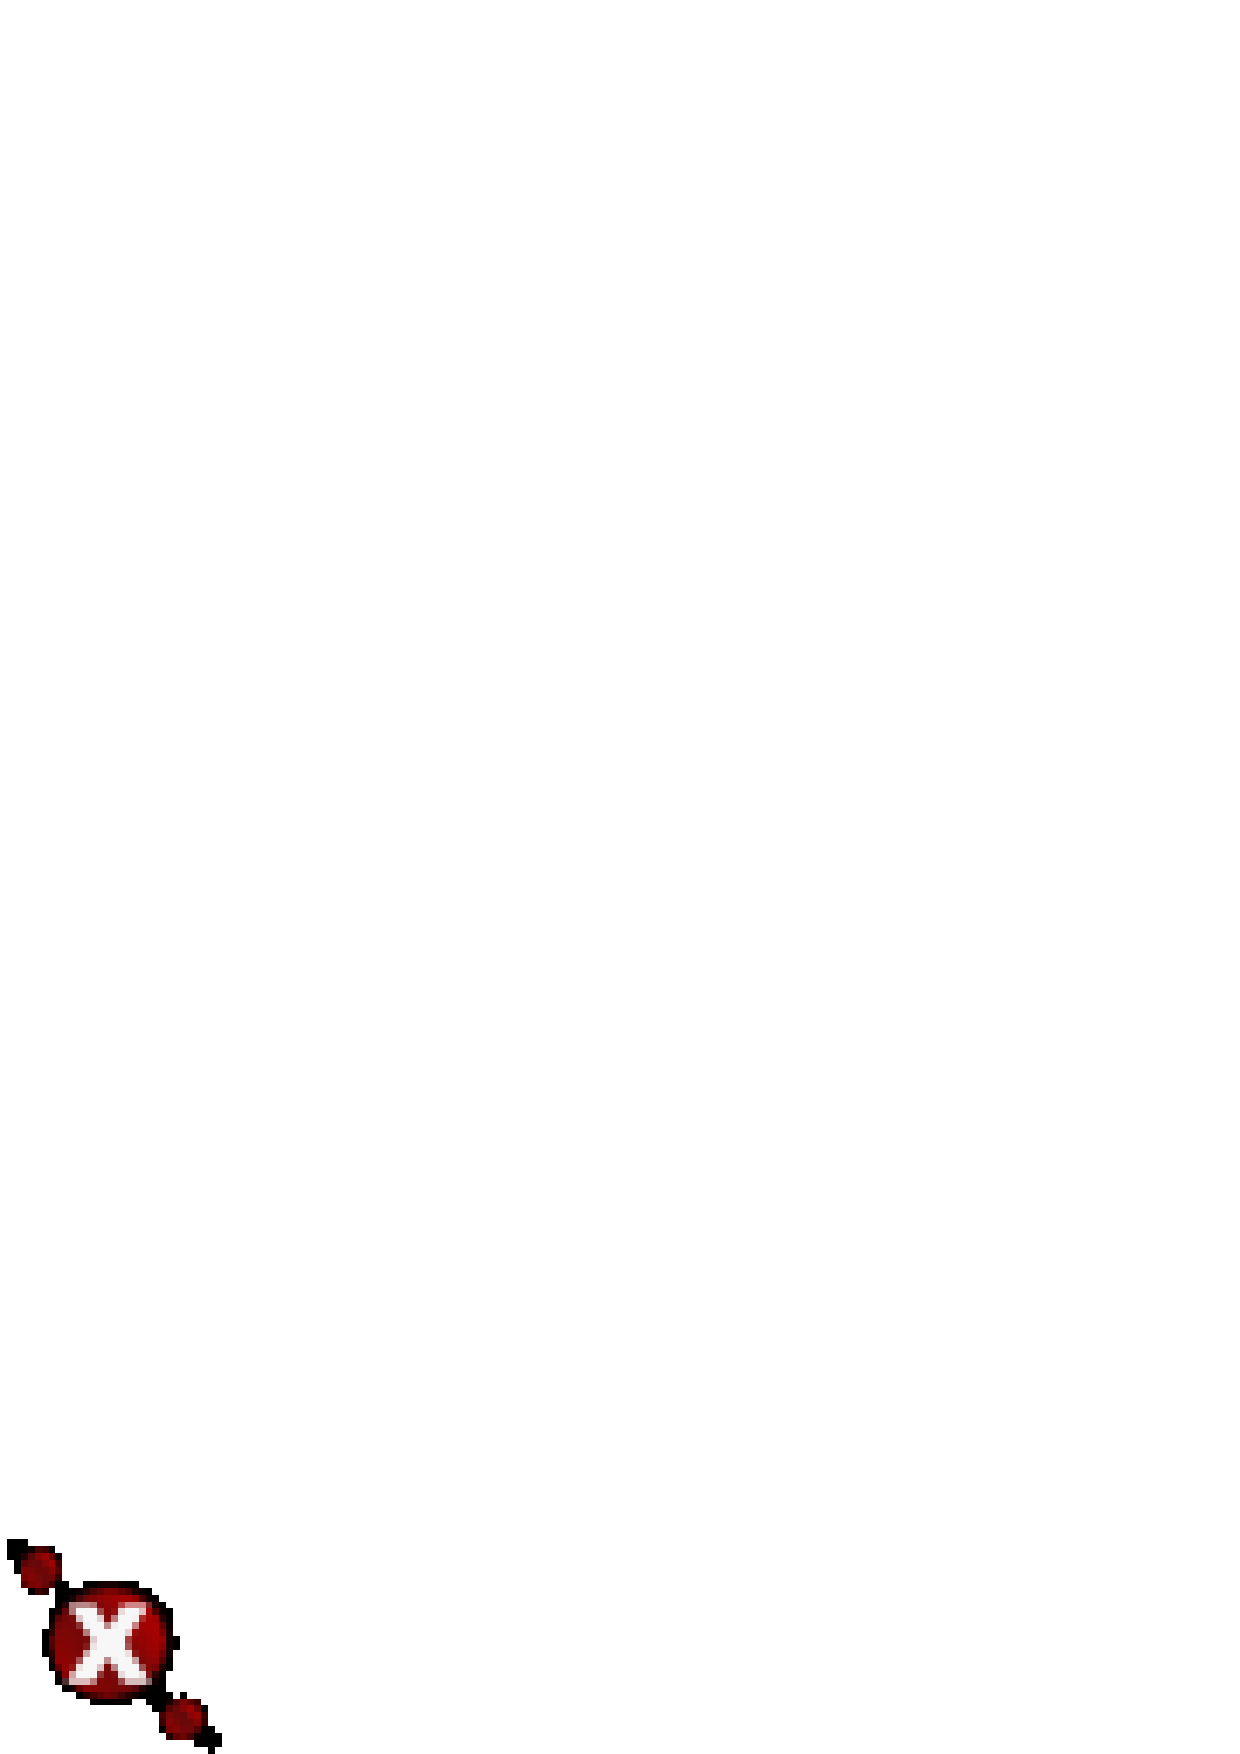
\includegraphics[width=0.7cm]{grass_delete_vertex} & Delete vertex & Delete vertex from existing line (confirm selected vertex by another click)\\
%\hline 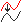
\includegraphics[width=0.7cm]{grass_move_line} & Move element & Move selected boundary, line, point or centroid and click on new position\\
%\hline 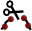
\includegraphics[width=0.7cm]{grass_split_line} & Split line & Split an existing line to 2 parts\\
%\hline 
\includegraphics[width=0.7cm]{grass_delete_line} & Delete element & Delete existing boundary, line, point or centroid (confirm selected element by another click)\\
%\hline 
\includegraphics[width=0.7cm]{grass_edit_attributes} & Edit attributes & Edit attributes of selected element (note that one element can represent more features, see above)\\
%\hline 
\includegraphics[width=0.7cm]{grass_close_edit} & Close & Close session and save current status (rebuilds topology afterwards)\\
\hline \textbf{Ic\^one} & \textbf{Outil} & \textbf{Fonction} \\
\hline 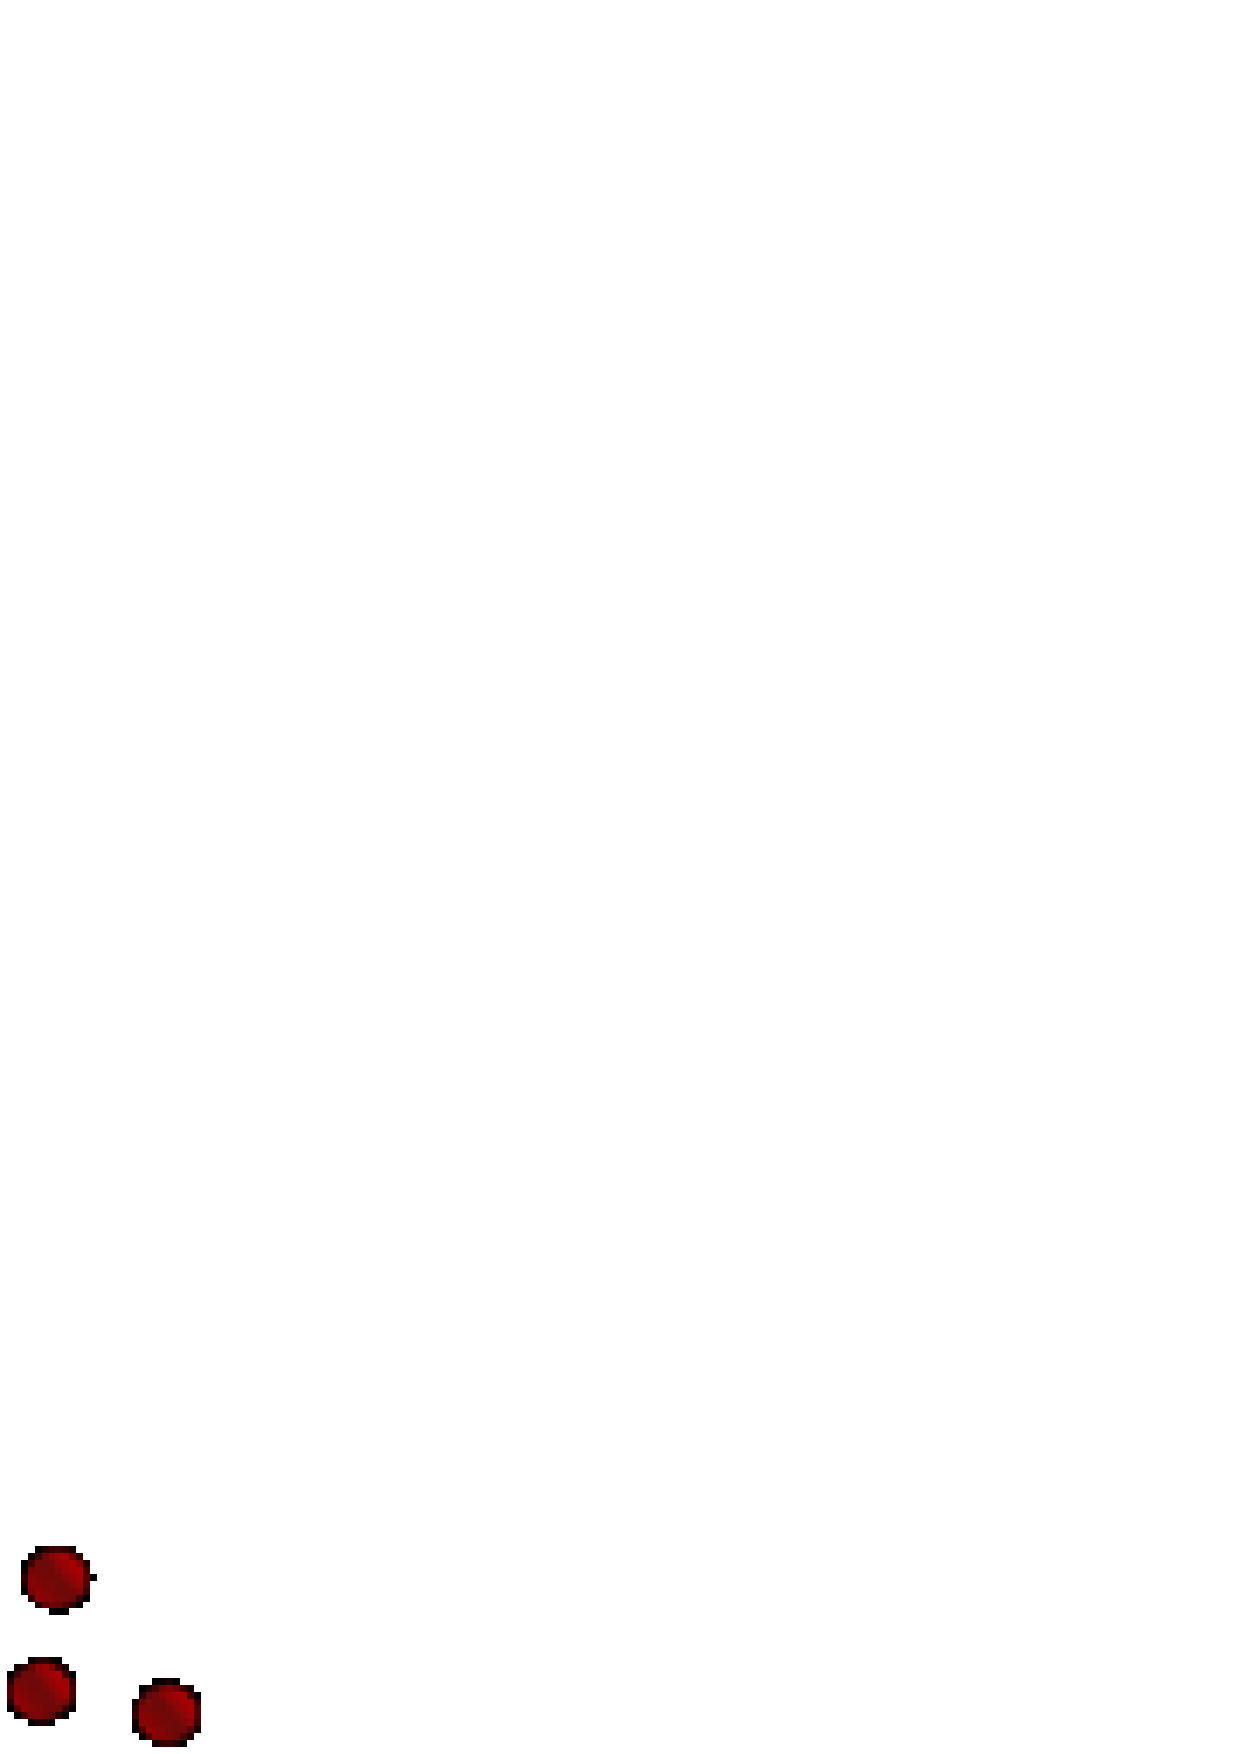
\includegraphics[width=0.7cm]{grass_new_point} & Nouveau Point & Num\'erise un nouveau point \\
\hline 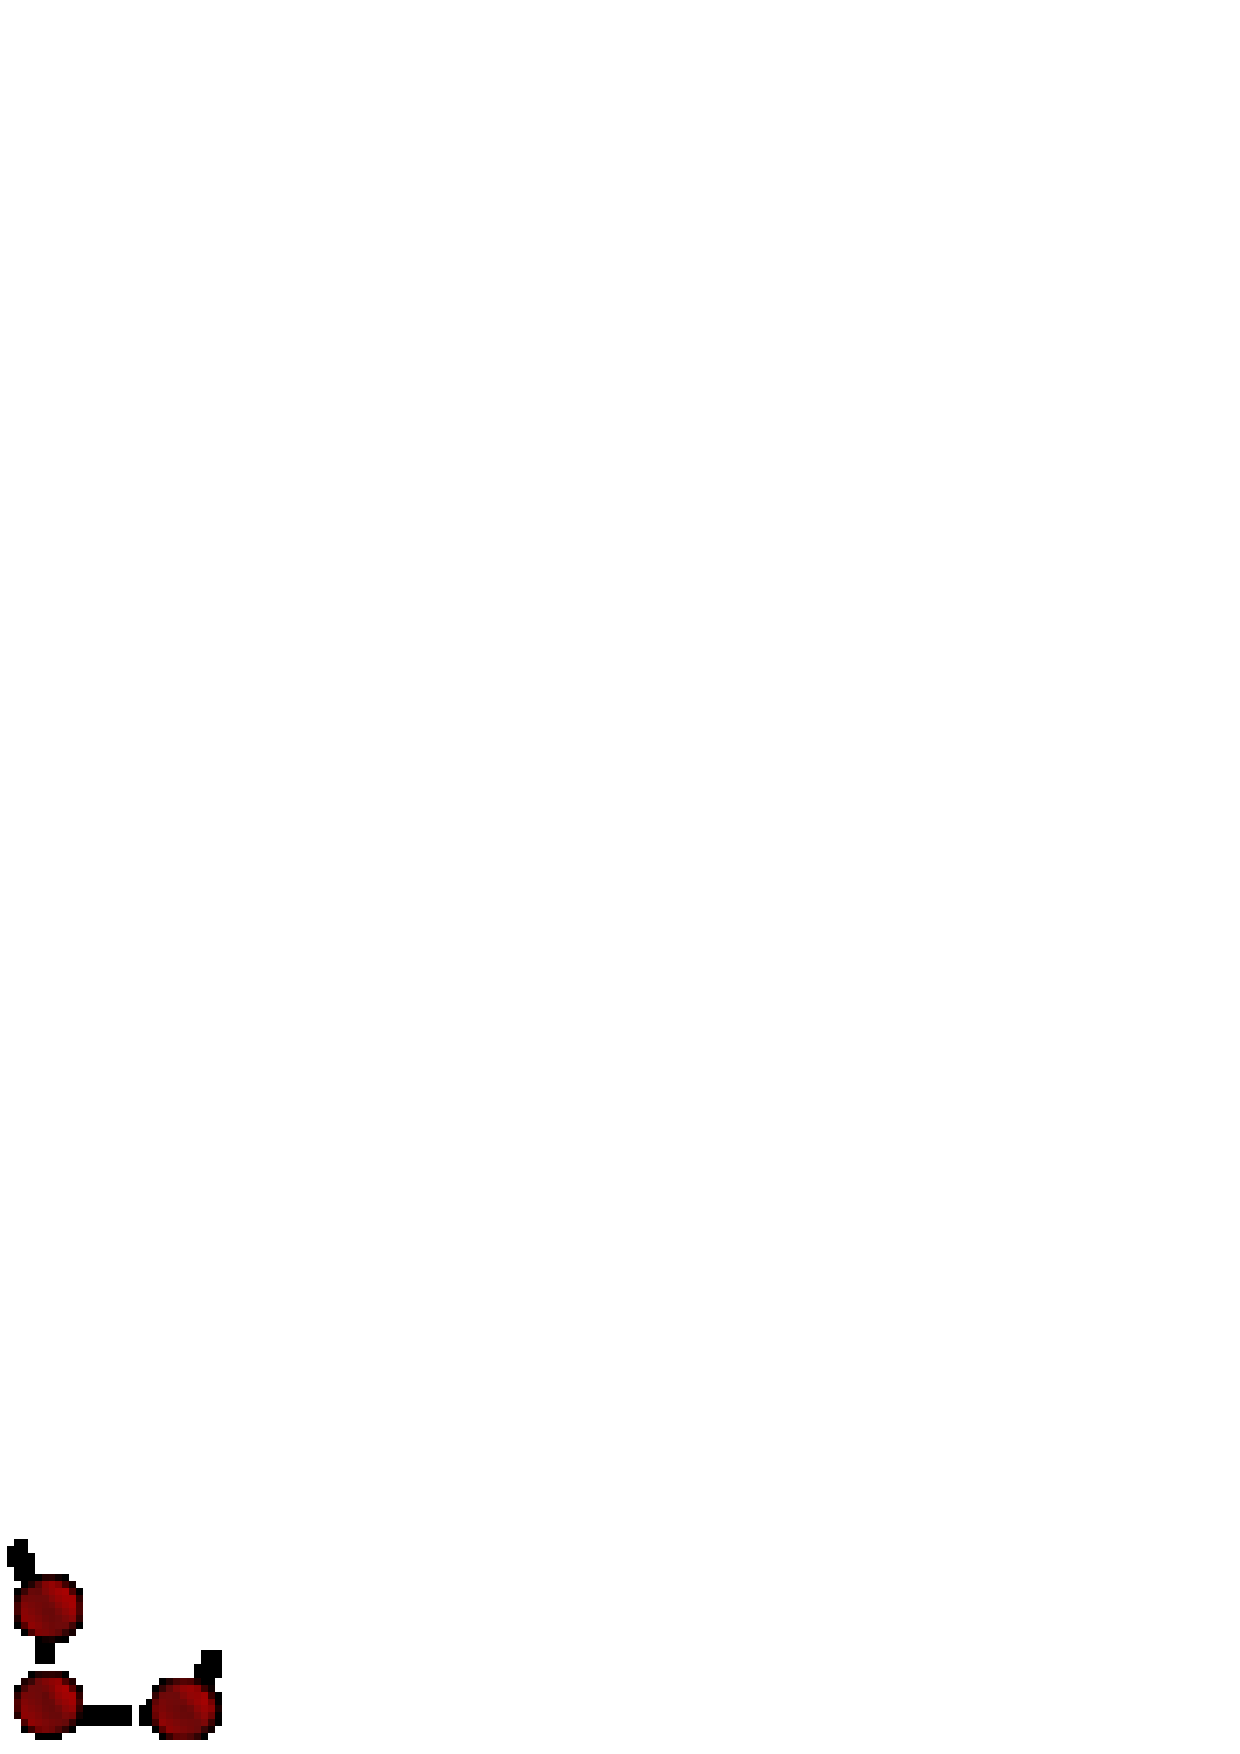
\includegraphics[width=0.7cm]{grass_new_line} & Nouvelle Ligne & Num\'erise une nouvelle ligne (terminez la num\'erisation en s\'electionnant un nouvel outil) \\
\hline 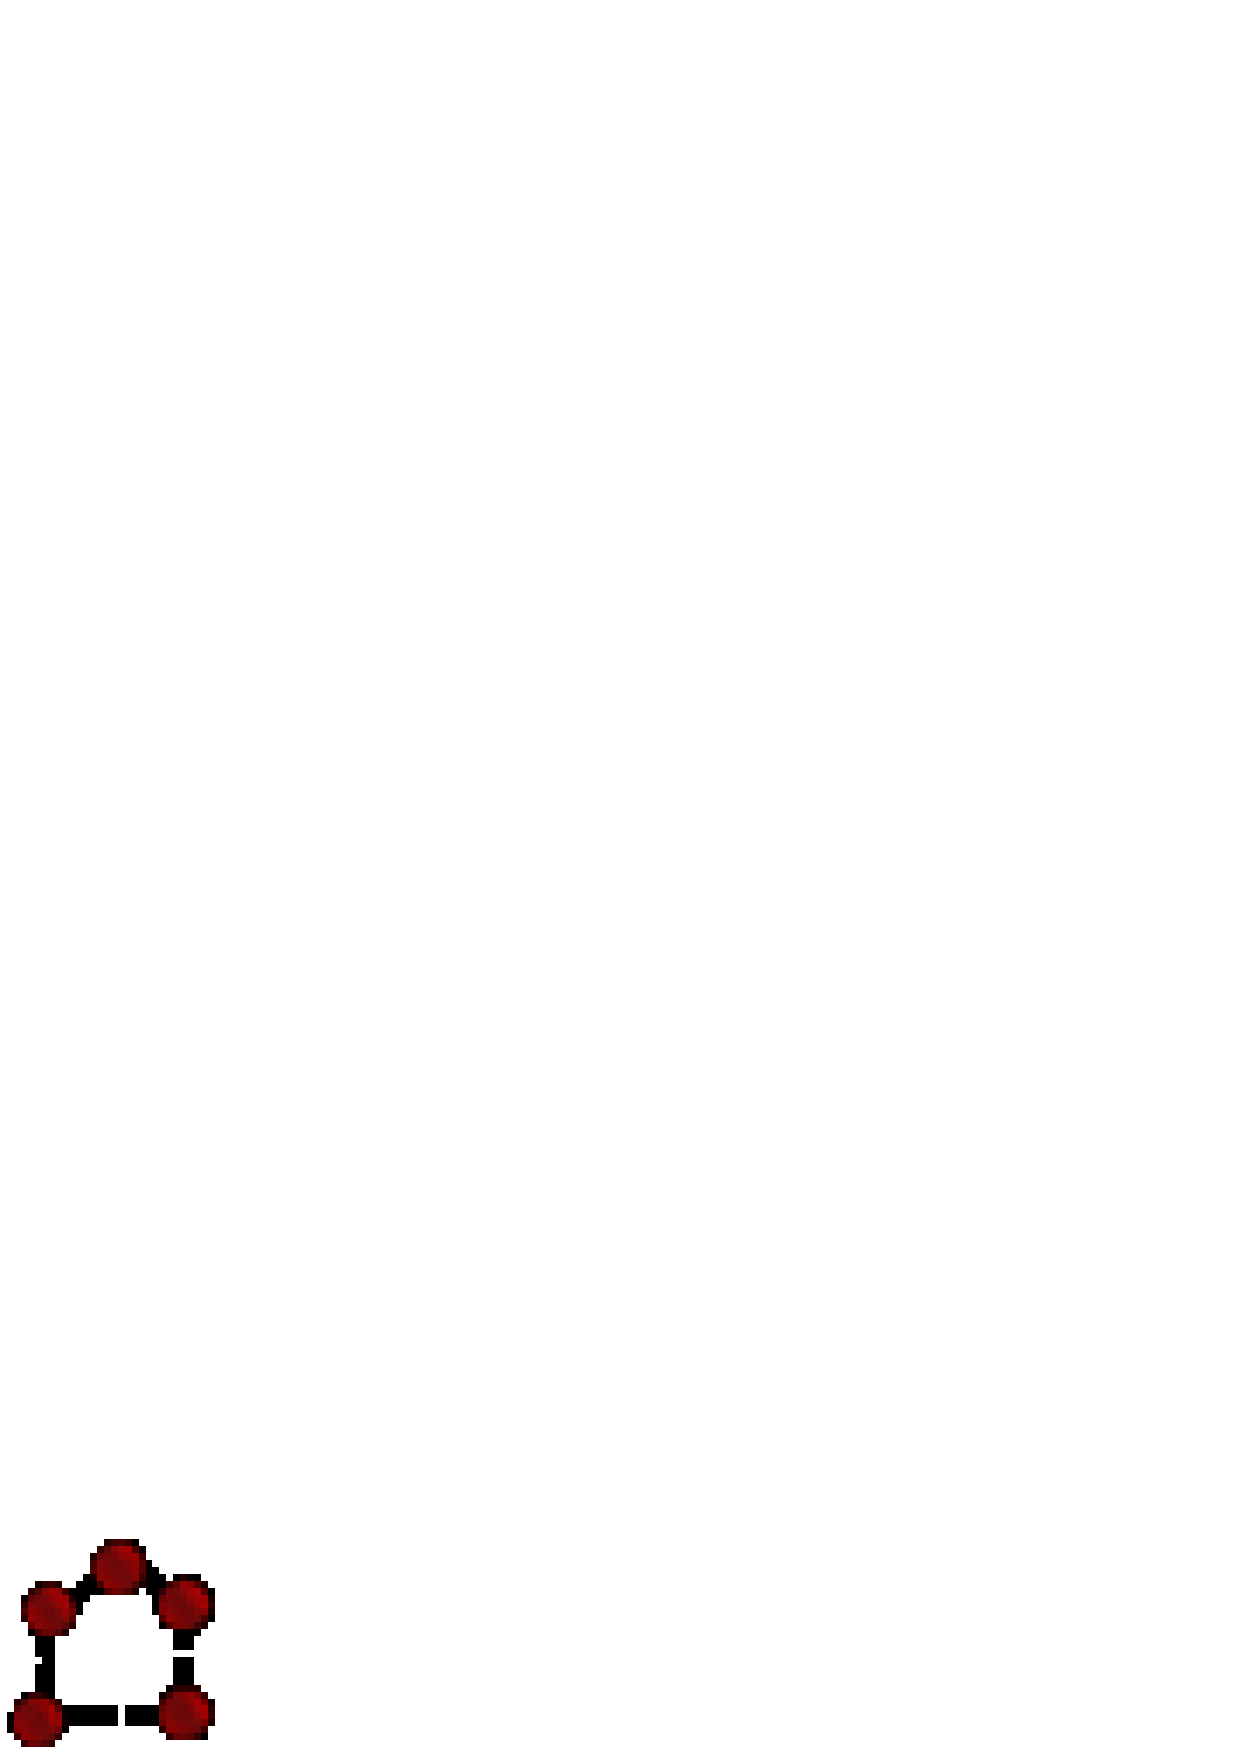
\includegraphics[width=0.7cm]{grass_new_boundary} & Nouveau Contour & Num\'erise un nouveau contour (terminer la num\'erisation en s\'electionnant un nouvel outil)\\
\hline 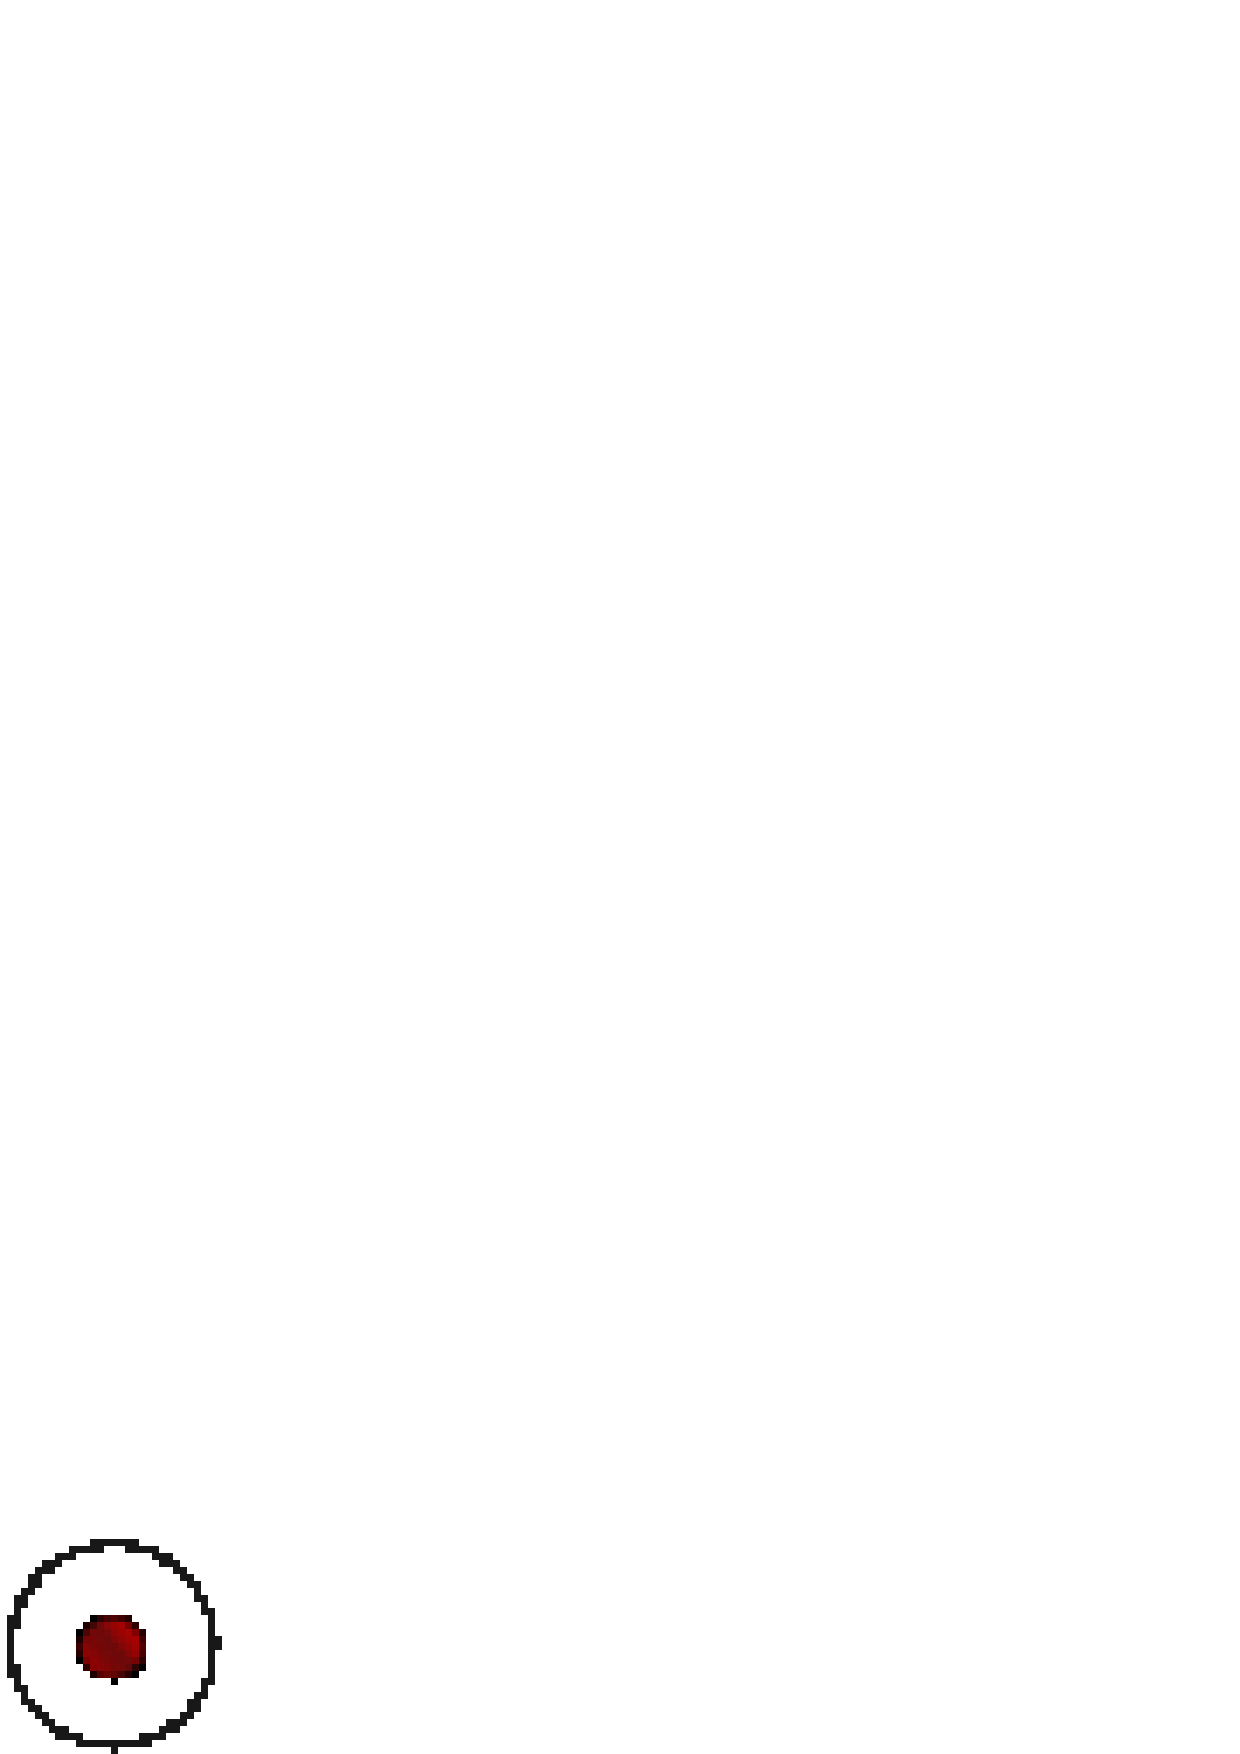
\includegraphics[width=0.7cm]{grass_new_centroid} & Nouveau Centro"ide & Num\'erise un nouveau centro"ide (emplacement de l'\'etiquette d'un polygone existant)\\
\hline 
\includegraphics[width=0.7cm]{grass_move_vertex} & D\'eplacer le sommet & D\'eplace un sommet d'une ligne ou d'un polygone existant et indique sa nouvelle position\\
\hline 
\includegraphics[width=0.7cm]{grass_add_vertex} & Ajouter un sommet & Ajoute un nouveau sommet \`a une ligne existante\\
\hline 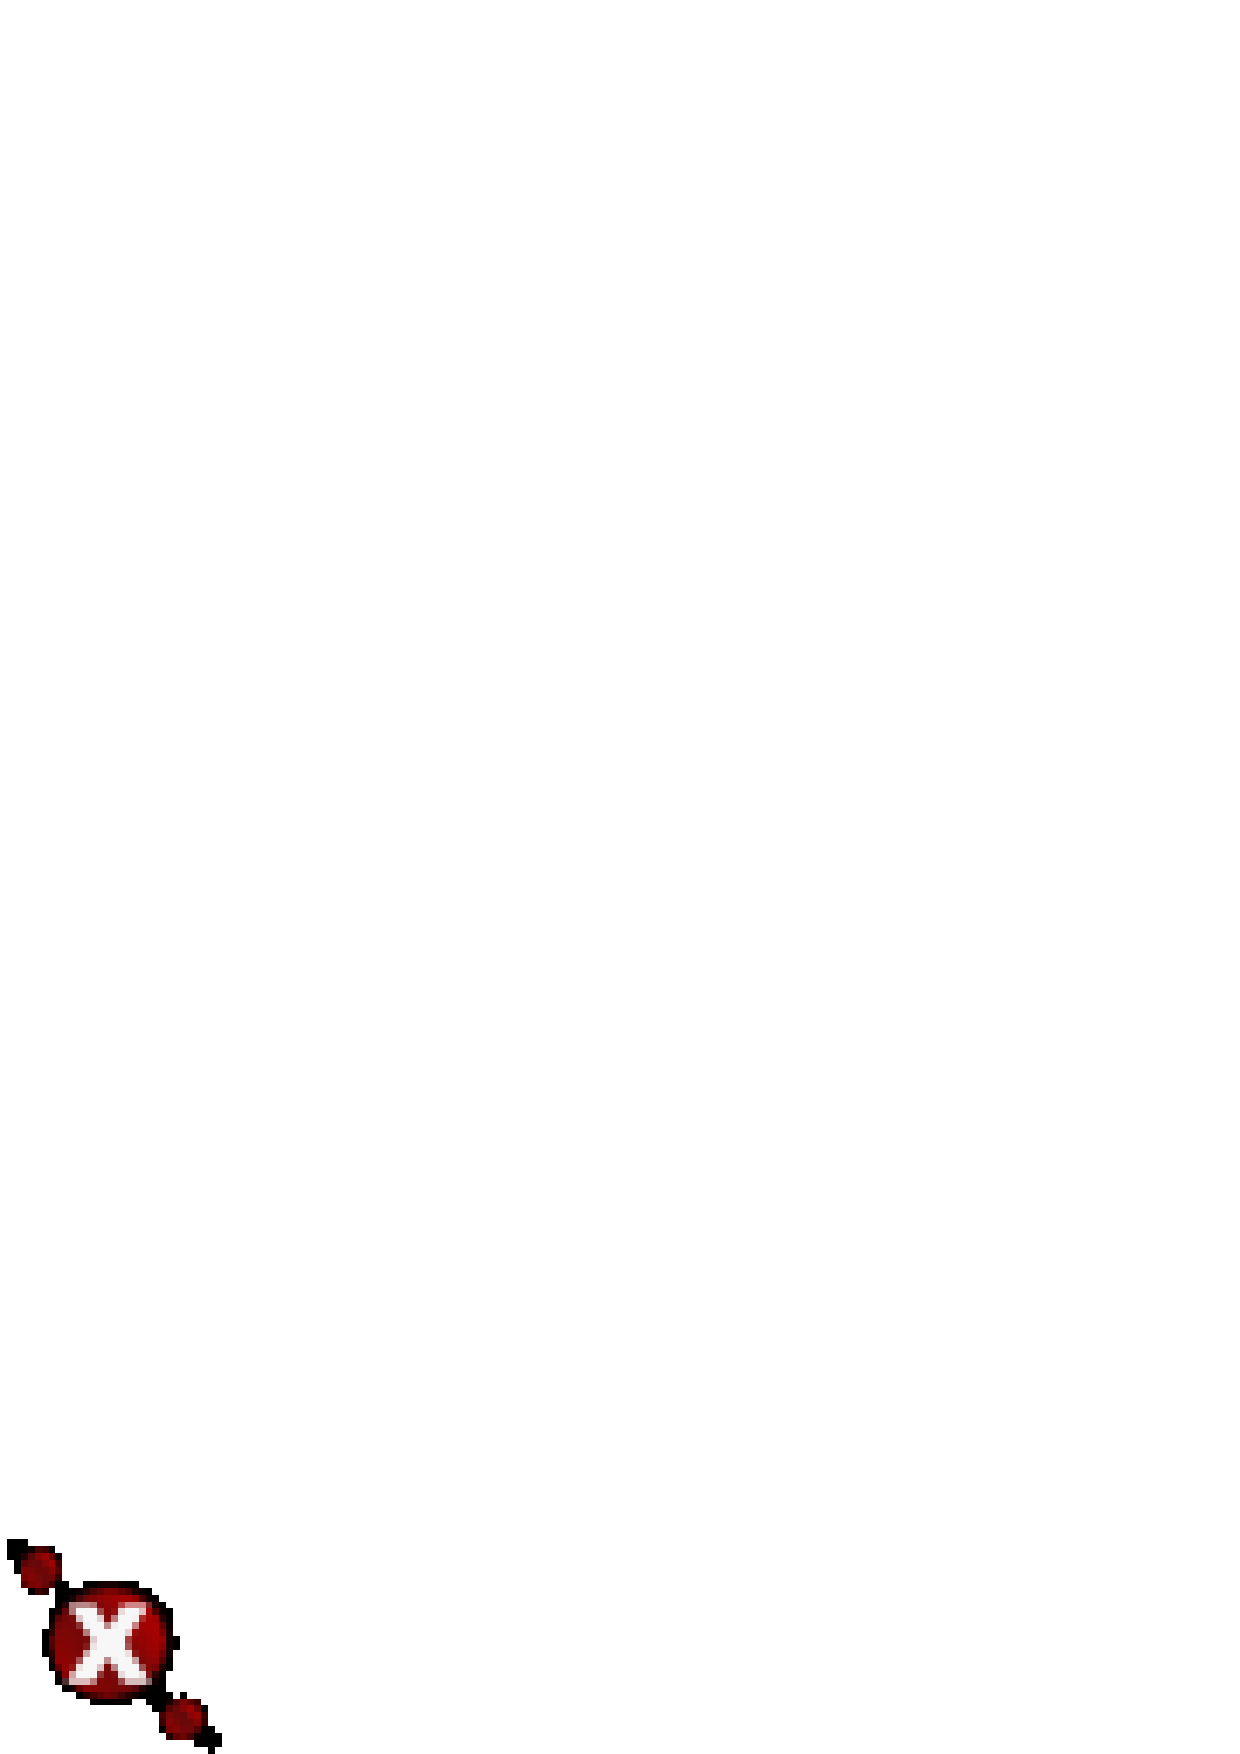
\includegraphics[width=0.7cm]{grass_delete_vertex} & Effacer un sommet & Efface un sommet d'une ligne existante (confirmez le sommet s\'electionn\'e avec un autre clic)\\
\hline 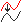
\includegraphics[width=0.7cm]{grass_move_line} & D\'eplace l'\'el\'ement & D\'eplacez la limite, la ligne, le point ou le centro"ide s\'electionn\'e puis cliquez sur la nouvelle position\\
\hline 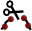
\includegraphics[width=0.7cm]{grass_split_line} & Coupe la ligne & Coupe une ligne existante en deux parties\\
\hline 
\includegraphics[width=0.7cm]{grass_delete_line} & Efface l'\'el\'ement & Efface une limite, une ligne, un point ou un centro"ide existant (confirmez l'\'el\'ement s\'electionn\'e avec un autre clic)\\
\hline 
\includegraphics[width=0.7cm]{grass_edit_attributes} & \'Editer les attributs & \'Edite les attributs de l'\'el\'ement s\'electionn\'e (notez qu'un seul \'el\'ement peut repr\'esenter plusieurs g\'eom\'etries, voir ci-dessus)\\
\hline 
\includegraphics[width=0.7cm]{grass_close_edit} & Fermer & Ferme la session et sauvegarde l'\'etat actuel (reconstruit la topologie apr\`es)\\
\hline
\end{tabular}
\end{table}

%\minisec{Category Tab}\index{GRASS!category settings}
\minisec{Onglet Categorie}\index{GRASS!param\`etres de cat\'egorie}
%The \tab{Category} tab allows you to define the way in which the category values will be assigned to a new geometry element.
L'onglet \tab{Categorie} vous permet de d\'efinir la mani\`ere dont les valeurs du champ category sont assign\'ees au nouvel \'el\'ement g\'eom\'etrique.

\begin{figure}[h]
 \begin{center}
  %\caption{GRASS Digitizing Category Tab \nixcaption}\label{fig:grass_digitizing_category}
  \caption{Onglet Cat\'egorie d'\'Edition GRASS \nixcaption}\label{fig:grass_digitizing_category}
  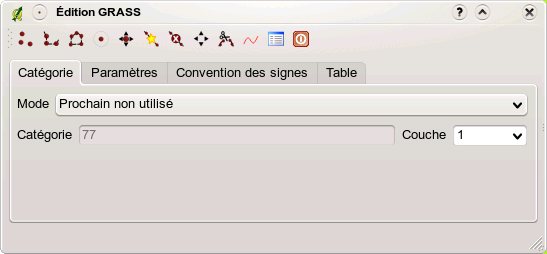
\includegraphics[clip=true,width=10cm]{grass_digitizing_category}
 \end{center}
\end{figure}

\begin{itemize}
%\item \textbf{Mode}: what category value shall be applied to new geometry elements.
\item \textbf{Mode}: quelle cat\'egorie sera appliqu\'e au nouvel \'el\'ement.
\begin{itemize}
%\item Next not used - apply next not yet used category value to geometry element.
\item Prochain non utilis\'e - applique la valeur suivante non utilis\'ee du champ category \`a l'\'el\'ement g\'eom\'etrique.
%\item Manual entry - manually define the category value for the geometry element in the 'Category'-entry field.
\item Saisie manuelle - saisir manuellement la valeur du champ category pour l'\'el\'ement g\'eom\'etrique.
%\item No category - Do not apply a category value to the geometry element. This is e.g. used for area boundaries, because the category values are connected via the centroid.
\item Pas de cat\'egorie - ne pas remplir le champ category. C'est par exemple utilis\'e pour les surfaces car les valeurs de cat\'egorie sont stock\'ees via le centro"ide
\end{itemize}
%\item \textbf{Category} - A number (ID) is attached to each digitized geometry element. It is used to connect each geometry element with its attributes.
\item \textbf{Categorie} - un identifiant (ID) est attach\'e \`a chaque objet num\'eris\'e. Il est utilis\'e pour connecter les objets g\'eom\'etriques avec ces attributs.
%\item \textbf{Field (layer)} - Each geometry element can be connected with several attribute tables using different GRASS geometry layers. Default layer number is 1. 
\item \textbf{Couche} - Chaque objet peut \^etre connect\'e \`a diff\'erentes tables attributaires au travers des diff\'erentes sous-couches. Le num\'ero de sous-couche par d\'efaut est 1.

\end{itemize}

%\begin{Tip}\caption{\textsc{Creating an additional GRASS 'layer' with QGIS}}
\begin{Astuce}\caption{\textsc{Cr\'eation d'une sous-couche suppl\'ementaire avec QGIS}}
%\qgistip{If you would like to add more layers to your dataset, just add a new number in the 'Field (layer)' entry box and press return. 
%In the Table tab you can create your new table connected to your new layer.
\qgistip{Si vous souhaitez avoir plusieurs sous-couches dans votre couche vecteur, ajouter simplement un nouveau chiffre dans la zone de saisie 'Couche' et appuyez sur entr\'ee. Dans l'onglet Table, vous pouvez cr\'eer de nouvelles tables attributaires connect\'ees \`a votre nouvelle sous-couche.
}
\end{Astuce}

\minisec{Onglet Param\`etres}\label{label_settingtab}\index{GRASS!tol\'erance d'accrochage}

%The \tab{Settings} tab allows you to set the snapping in screen pixels. The threshold defines at what distance new points or line ends are snapped to
%existing nodes. This helps to prevent gaps or dangles between boundaries. The default is set to 10 pixels.
L'onglet \tab{Param\`etres} vous permet de d\'efinir la tol\'erance d'accrochage en pixels \'ecran. Le seuil d\'efinit \`a partir de quelle distance les nouveaux points ou les nouvelles lignes sont accroch\'ees automatiquement \`a des noeuds existants. Cela aide \`a \'eviter de cr\'eer des trous ou des superpositions entre les contours. La valeur par d\'efaut est fix\'ee \`a 10 pixels.

\begin{figure}[h]
 \begin{center}
% \caption{GRASS Digitizing Settings Tab \nixcaption}\label{fig:grass_digitizing_settings}
 \caption{Onglet Param\`etres d'\'Edition GRASS \nixcaption}\label{fig:grass_digitizing_settings}
 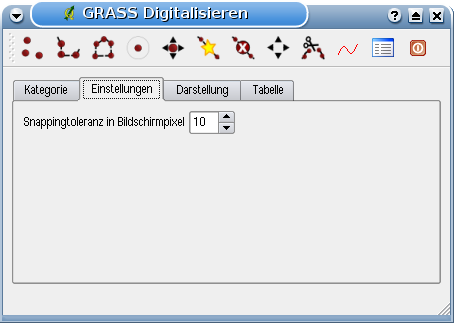
\includegraphics[clip=true,width=8cm]{grass_digitizing_settings}
 \end{center}
\end{figure}

%\minisec{Symbology Tab}\index{GRASS!symbology settings}
\minisec{Onglet Convention des signes}\index{GRASS!convention des signes}

%The \tab{Symbology} tab allows you to view and set symbology and color settings for various geometry types and their topological status (e.g. closed / opened boundary).
L'onglet \tab{Convention des signes} vous permet d'afficher et modifier la symbologie, la couleur des diff\'erentes formes g\'eom\'etriques ainsi que leur statut topologique (par exemple : contour ouvert / ferm\'e)

\begin{figure}[h]
 \begin{center}
 %\caption{GRASS Digitizing Symbolog Tab \nixcaption}\label{fig:grass_digitizing_symbology}
 \caption{Onglet Convention des signes d'\'Edition GRASS \nixcaption}\label{fig:grass_digitizing_symbology}
 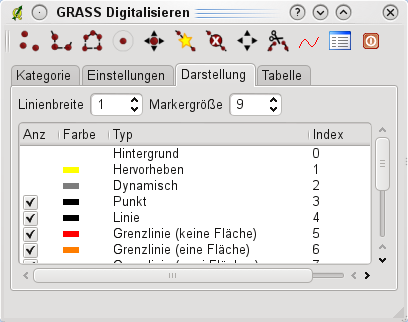
\includegraphics[clip=true,width=8cm]{grass_digitizing_symbology}
 \end{center}
\end{figure}

%\minisec{Table Tab} \index{GRASS!table editing}
\minisec{Onglet Table} \index{GRASS!\'Editer une table}
%The \tab{Table} tab provides information about the database table for a given 'layer'. Here you can add new columns to an existing attribute table,
%or create a new database table for a new GRASS vector layer (see Section \ref{sec:creating_new_grass_vectors}).
L'onglet \tab{Table} donne des informations sur la table attributaire d'une sous-couche donn\'ee. C'est ici que vous pouvez ajouter des colonnes \`a une table attributaire existante ou cr\'eer une nouvelle table attributaire pour une nouvelle couche vectorielle GRASS (voir Section \ref{sec:creating_new_grass_vectors}).

\begin{figure}[h]
 \begin{center}
% \caption{GRASS Digitizing Table Tab \nixcaption}\label{fig:grass_digitizing_table}
 \caption{Onglet Table du mode \'Edition GRASS \nixcaption}\label{fig:grass_digitizing_table}
 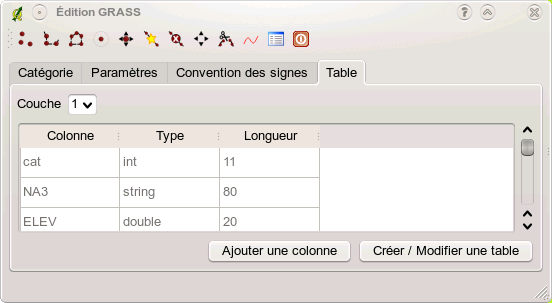
\includegraphics[clip=true,width=10cm]{grass_digitizing_table}
 \end{center}
\end{figure}

\begin{Astuce}\caption{\textsc{\'Editer les permissions GRASS}}\index{GRASS!\'editer les permissions}
%\qgistip{You must be the owner of the GRASS \filename{MAPSET} you want to edit. It is impossible to edit data layers in a \filename{MAPSET} that is not yours, even if you have write permissions.
\qgistip{Vous devez \^etre propri\'etaire du \filename{Jeu de donn\'ees} que vous voulez \'editer. Il est impossible de modifier des informations d'un \filename{Jeu de donn\'ees} qui n'est pas \`a vous, m\^eme si vous avez des droits en \'ecriture.
}
\end{Astuce} 

%\subsection{The GRASS region tool}\label{sec:grass_region}\index{GRASS!region}
\subsection{L'outil r\'egion GRASS}\label{sec:grass_region}\index{GRASS!r\'egion}

%The region definition (setting a spatial working window) in GRASS is important for working with raster layers. Vector analysis is per default not limited to any defined region definitions. All newly-created rasters will have the spatial extension and resolution of the currently defined GRASS region, regardless of their original extension and resolution. The current GRASS region is stored in the \filename{\$LOCATION/\$MAPSET/WIND} file, and it defines north, south, east and west bounds, number of columns and rows, horizontal and vertical spatial resolution.
La d\'efinition d'une r\'egion (d\'efinir une emprise spatiale de travail) dans GRASS est tr\`es importante pour travailler avec des couches rasters. Le travail d'analyse vecteur n'est, par d\'efaut, pas limit\'ee \`a une r\'egion d\'efinie. Tous les rasters nouvellement cr\'e\'es auront l'extension spatiale et la r\'esolution de la r\'egion GRASS en cours d'utilisation, ind\'ependamment de leur extension et r\'esolution d'origine. La r\'egion courante GRASS est stock\'ee dans le fichier \filename{\$LOCATION/\$MAPSET/WIND}, et celui-ci d\'efinit les limites Nord, Sud, Est et Ouest, le nombre de lignes et de colonnes ainsi que la r\'esolution spatiale horizontale et verticale.

%It is possible to switch on/off the visualization of the GRASS region in the QGIS canvas using the \toolbtntwo{grass_region}{Display current GRASS region} button. \index{GRASS!region!display}.
Il est possible de d'afficher ou de masquer l'affichage de la r\'egion GRASS dans QGIS \`a l'aide du bouton\toolbtntwo{grass_region}{Afficher la r\'egion courante GRASS}. \index{GRASS!r\'egion!afficher}.

%With the \toolbtntwo{grass_region_edit}{Edit current GRASS region} icon you can open a dialog to change the current region and the symbology of the GRASS region rectangle in the QGIS canvas. Type in the new region bounds and resolution and click \button{OK}. It also allows to select a new region interactively with your mouse on the QGIS canvas. Therefore click with the left mouse button in the QGIS canvas, open a rectangle, close it using the left mouse button again and click \button{OK}.\index{GRASS!region!editing} The GRASS module \filename{g.region} provide a lot more parameters to define an appropriate region extend and resolution for your raster analysis. You can use these parameters with the GRASS Toolbox, described in Section \ref{subsec:grass_toolbox}.
A l'aide du bouton \toolbtntwo{grass_region_edit}{\'Editer la r\'egion courante GRASS} vous avez acc\`es \`a une bo\^ite dialogue qui vous permet de modifier la r\'egion courante ainsi que sa symbologie. Entrez les nouvelles limites et r\'esolution et cliquez sur \button{OK}. Cette bo\^ite de dialogue vous permet aussi de d\'efinir une nouvelle r\'egion interactivement \`a l'aide de la souris. Pour d\'efinir ce rectangle d'emprise, cliquez avec le bouton gauche de la souris et d\'efinissez un rectangle que vous terminerez en cliquant de nouveau sur le bouton gauche de la souris et fermez la bo\^ite de dialogue en cliquant sur \button{OK}.\index{GRASS!r\'egion!\'editer} Le module GRASS \filename{g.region} propose un grand nombre de param\`etres pour d\'efinir de fa\c{c}on appropri\'ee les limites et la r\'esolution d'une r\'egion pour faire de l'analyse raster. Vous pouvez vous servir de ces param\`etres dans la bo\^ite \`a outils GRASS d\'ecrite dans la section \ref{subsec:grass_toolbox}.



%\subsection{The GRASS toolbox}\label{subsec:grass_toolbox}\index{GRASS!toolbox}
\subsection{La bo\^ite \`a outils GRASS}\label{subsec:grass_toolbox}\index{GRASS!bo\^ite \`a outils} 

%The \toolbtntwo{grass_tools}{Open GRASS Tools} box provides GRASS module functionalities to work with data inside a selected GRASS \filename{LOCATION} and \filename{MAPSET}. To use the GRASS toolbox you need to open a \filename{LOCATION} and \filename{MAPSET} where you have write-permission (usually granted, if you created the \filename{MAPSET}). This is necessary, because new raster or vector layers created during analysis need to be written to the currently selected \filename{LOCATION} and \filename{MAPSET}.
La bo\^ite de dialogue \toolbtntwo{grass_tools}{Ouvrir les outils GRASS} donne acc\`es aux fonctionnalit\'es GRASS qui permettent de travailler dans un \filename{SECTEUR} et sur un \filename{Jeu de Donn\'ees}. Pour utiliser les outils GRASS, vous devez ouvrir un \filename{SECTEUR} et un \filename{Jeu de Donn\'ees} sur lequel vous avez des droits d'\'ecriture (que vous avez normalement si vous avez cr\'e\'e le \filename{Jeu de Donn\'ees}). Cela est n\'ecessaire car les rasters et les vecteurs nouvellement cr\'e\'es lors des analyses doivent \^etre \'ecrits dans le \filename{SECTEUR} et \filename{Jeu de Donn\'ees} courant.


%\subsubsection{Working with GRASS modules}\index{GRASS!toolbox}
\subsubsection{Travailler avec les modules GRASS}\index{GRASS!bo\^ite \`a outils} 

\begin{figure}[h]
\centering
%\caption{GRASS Toolbox and searchable Modules List \nixcaption}\label{fig:grass_modules}
%   \subfigure[Modules Tree] {\label{subfig:grass_module_tree}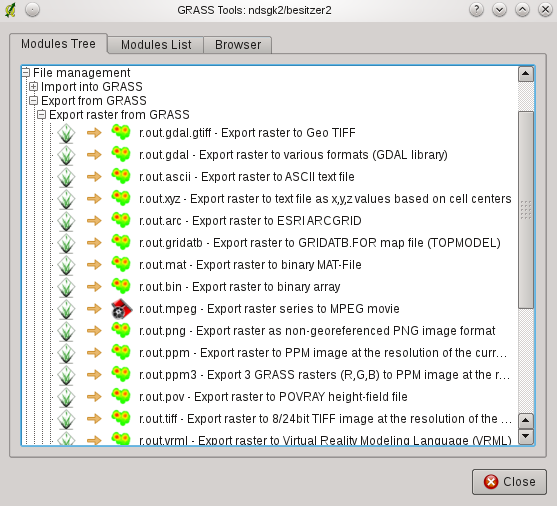
\includegraphics[clip=true, width=0.4\textwidth]{grass_toolbox_moduletree}}\goodgap
%   \subfigure[Searchable Modules List] {\label{subfig:grass_module_list}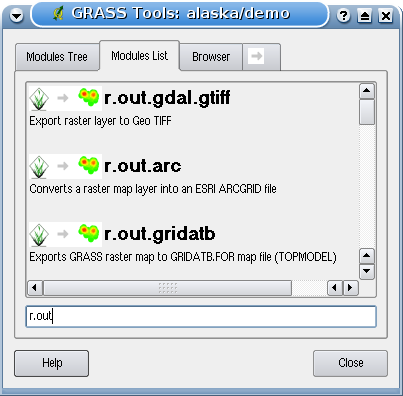
\includegraphics[clip=true, width=0.4\textwidth]{grass_toolbox_modulelist}}
\caption{Outils GRASS et Liste des Modules \nixcaption}\label{fig:grass_modules}
   \subfigure[Arborescence des modules] {\label{subfig:grass_module_tree}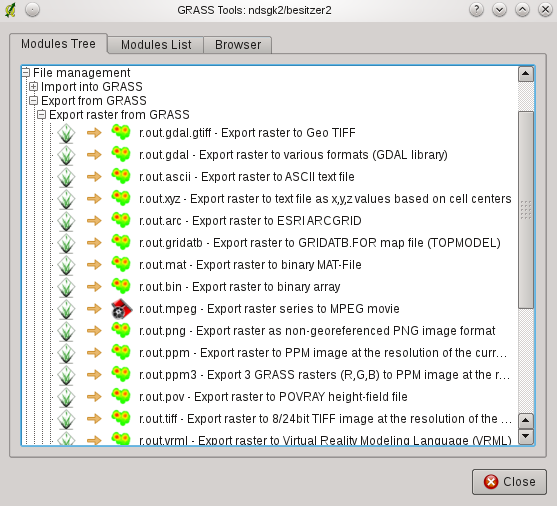
\includegraphics[clip=true, width=0.4\textwidth]{grass_toolbox_moduletree}}\goodgap
   \subfigure[Liste des modules avec possibilit\'e de recherche] {\label{subfig:grass_module_list}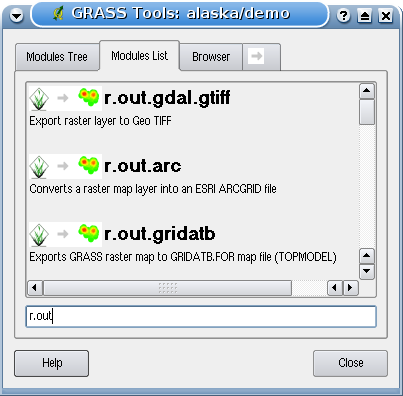
\includegraphics[clip=true, width=0.4\textwidth]{grass_toolbox_modulelist}}
\end{figure}

%The GRASS Shell inside the GRASS Toolbox provides access to almost all (more than 300) GRASS modules in command line modus. To offer a more user friendly working environment, about 200 of the available GRASS modules and functionalities are also provided by graphical dialogs. These dialogs are  grouped in thematic blocks, but are searchable as well. You find a complete list of GRASS modules available in QGIS version \CURRENT in appendix \ref{appdx_grass_toolbox_modules}. It is also possible to customize the GRASS Toolbox content. It is described in Section \ref{sec:toolbox-customizing}.
L'invite de commande de la bo\^ite \`a outils GRASS vous donne acc\`es \`a pratiquement tous les modules GRASS (pr\`es de 300) en ligne de commande. Afin d'offrir un environnement de travail plus agr\'eable, environ 200 d'entre eux sont fournis avec une bo\^ite de dialogue. Ces bo\^ites de dialogue sont group\'ees par th\`emes mais sont aussi accessibles par une recherche libre. Vous trouverez une liste compl\`ete des modules GRASS disponibles dans QGIS \CURRENT dans l'annexe \ref{appdx_grass_toolbox_modules}. Il est aussi possible de personnaliser le contenu de la bo\^ite \`a outils GRASS. Ceci est d\'ecrit dans la section \ref{sec:toolbox-customizing}.

%As shown in Figure \ref{fig:grass_modules}, you can look for the appropriate GRASS module using the thematically grouped \tab{Modules Tree} or the  searchable \tab{Modules List} tab. 
Comme indiqu\'e sur la figure \ref{fig:grass_modules}, vous pouvez chercher le module GRASS appropri\'e en utilisant l'onglet \tab{Arborescence des modules} ou en utilisant l'onglet \tab{Liste des Modules} pour faire une recherche.

%Clicking on a grapical module icon a new tab will be added to the toolbox dialog providing three new sub-tabs \tab{Options}, \tab{Output} and 
%\tab{Manual}. In Figure \ref{fig:grass_module_dialog} you see an example for the GRASS module \filename{v.buffer}.
Lorsque vous cliquez sur un module, un nouvel onglet appara\^it proposant trois sous-onglets \tab{Options}, \tab{Rendu} et \tab{Manuel}. Sur la figure \ref{fig:grass_module_dialog}, vous voyez un exemple pour le module GRASS \filename{v.buffer}.

\begin{figure}[h]
\centering
%\caption{GRASS Toolbox Module Dialogs \nixcaption}\label{fig:grass_module_dialog}
%   \subfigure[Module Options] {\label{subfig:grass_module_option}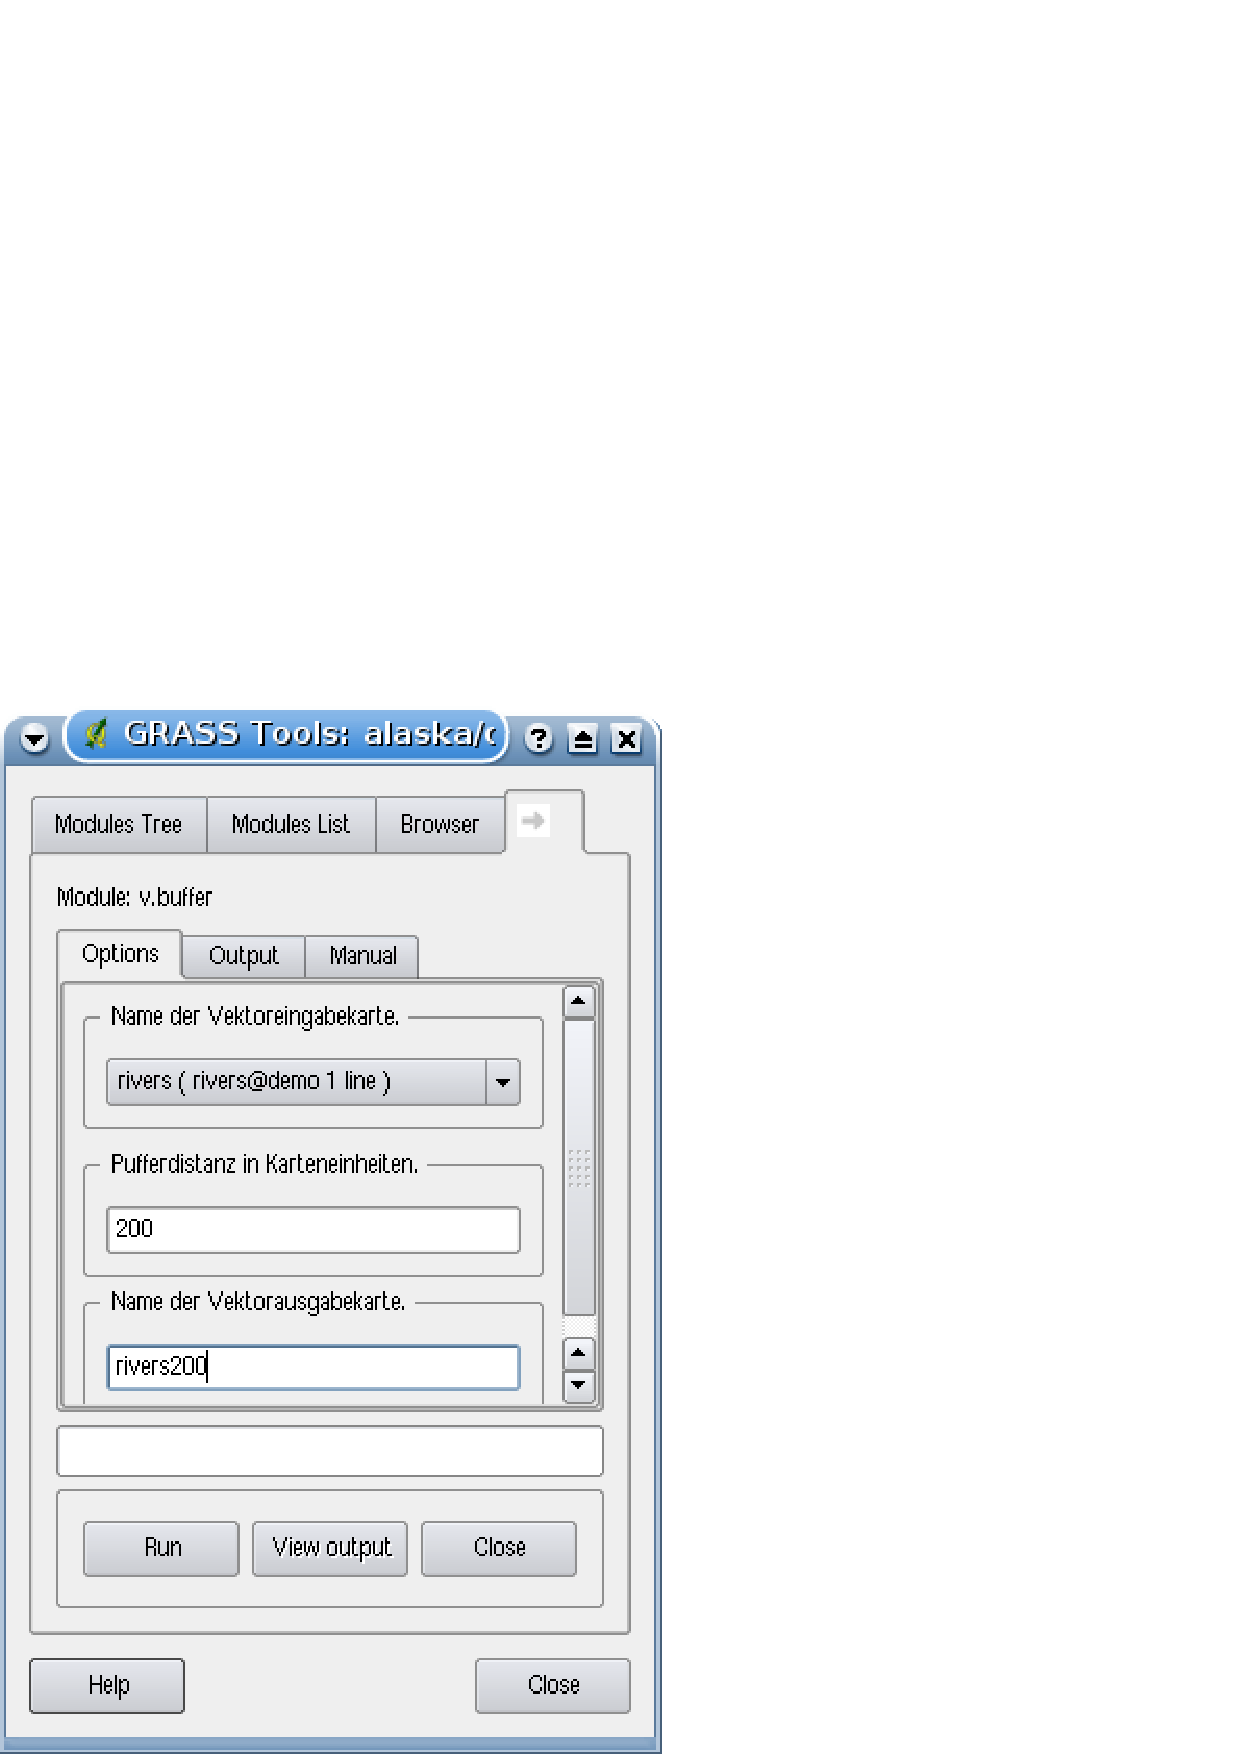
\includegraphics[clip=true, width=0.3\textwidth]{grass_module_option}}\goodgap
%   \subfigure[Modules Output] {\label{subfig:grass_module_output}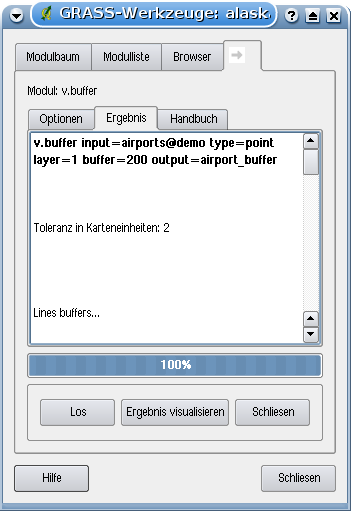
\includegraphics[clip=true, width=0.3\textwidth]{grass_module_output}}\goodgap
%   \subfigure[Module Manual] {\label{subfig:grass_module_manual}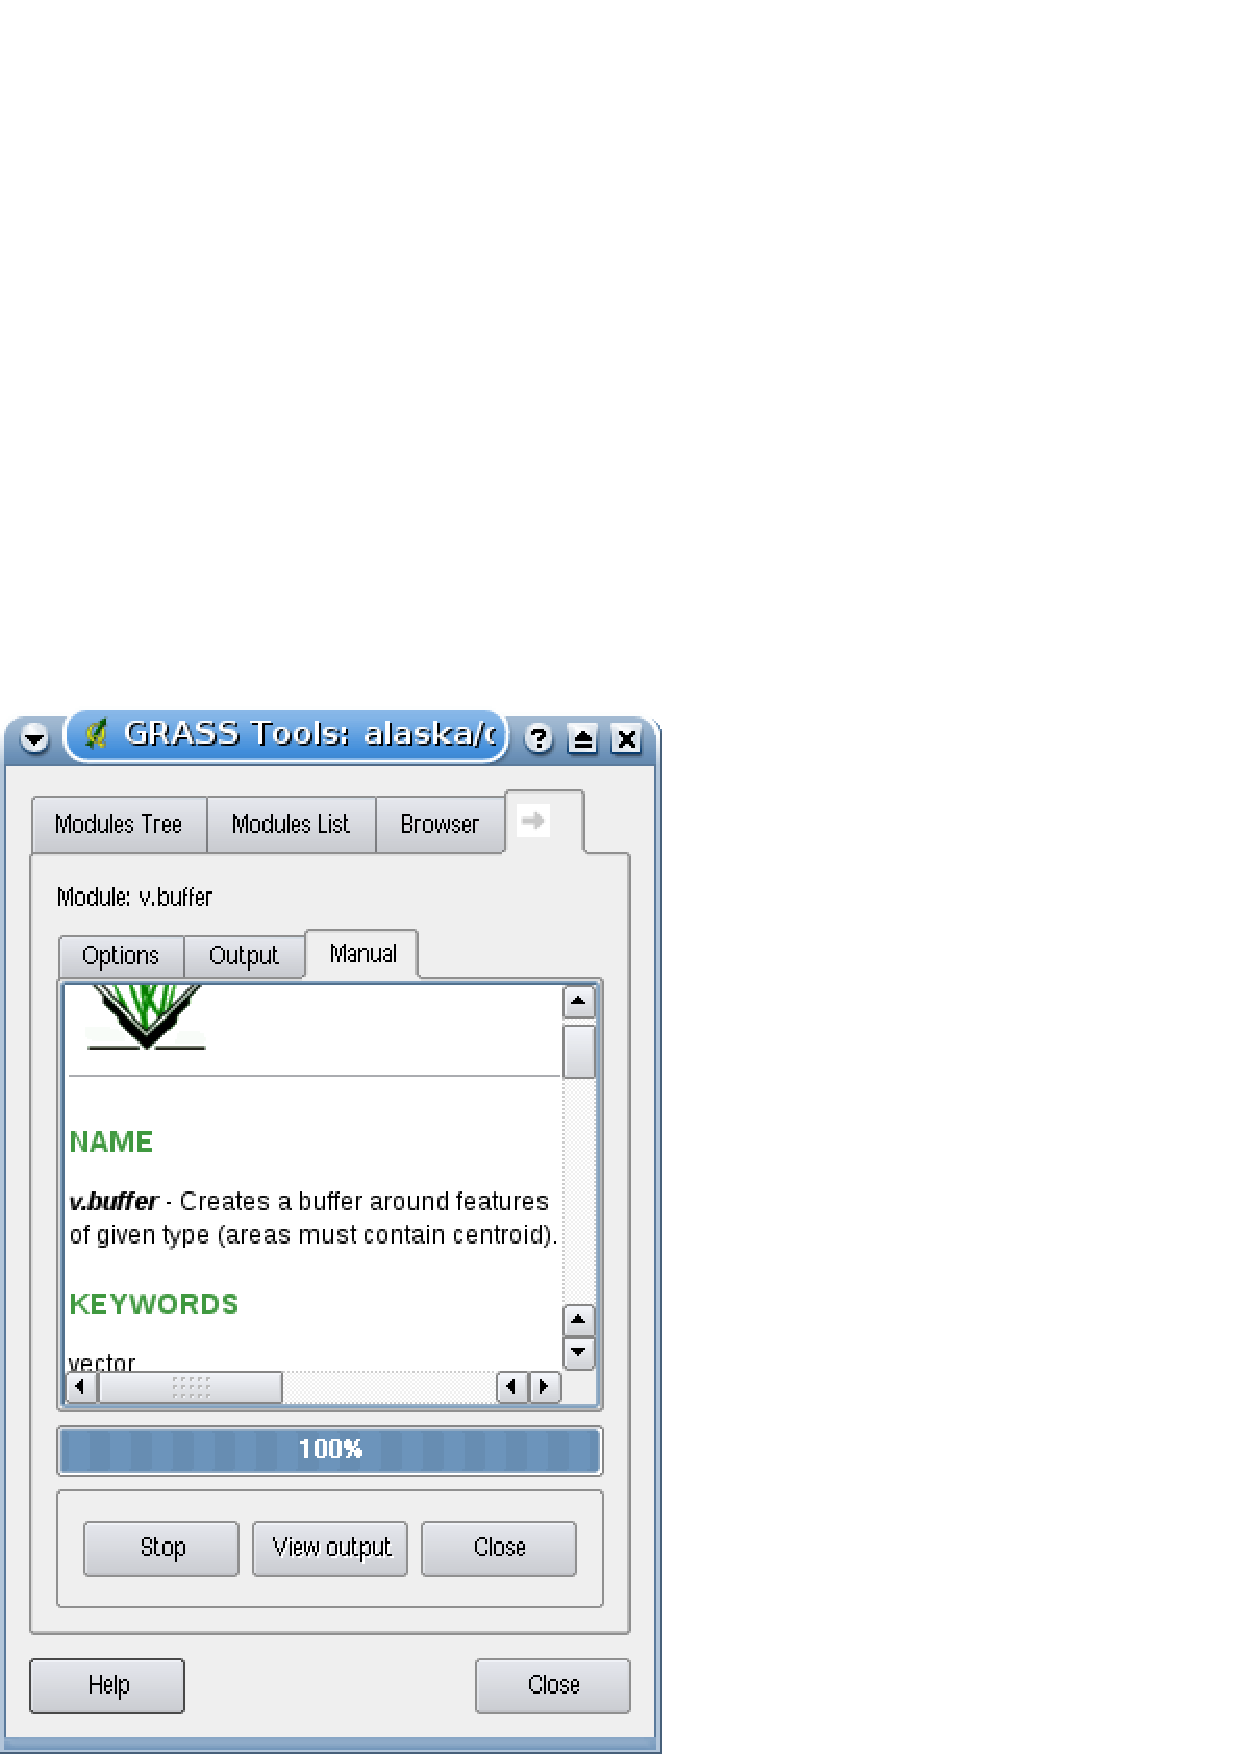
\includegraphics[clip=true, width=0.3\textwidth]{grass_module_manual}}
\caption{Bo\^ite de dialogue d'un module issue des outils GRASS \nixcaption}\label{fig:grass_module_dialog}
   \subfigure[Options du module] {\label{subfig:grass_module_option}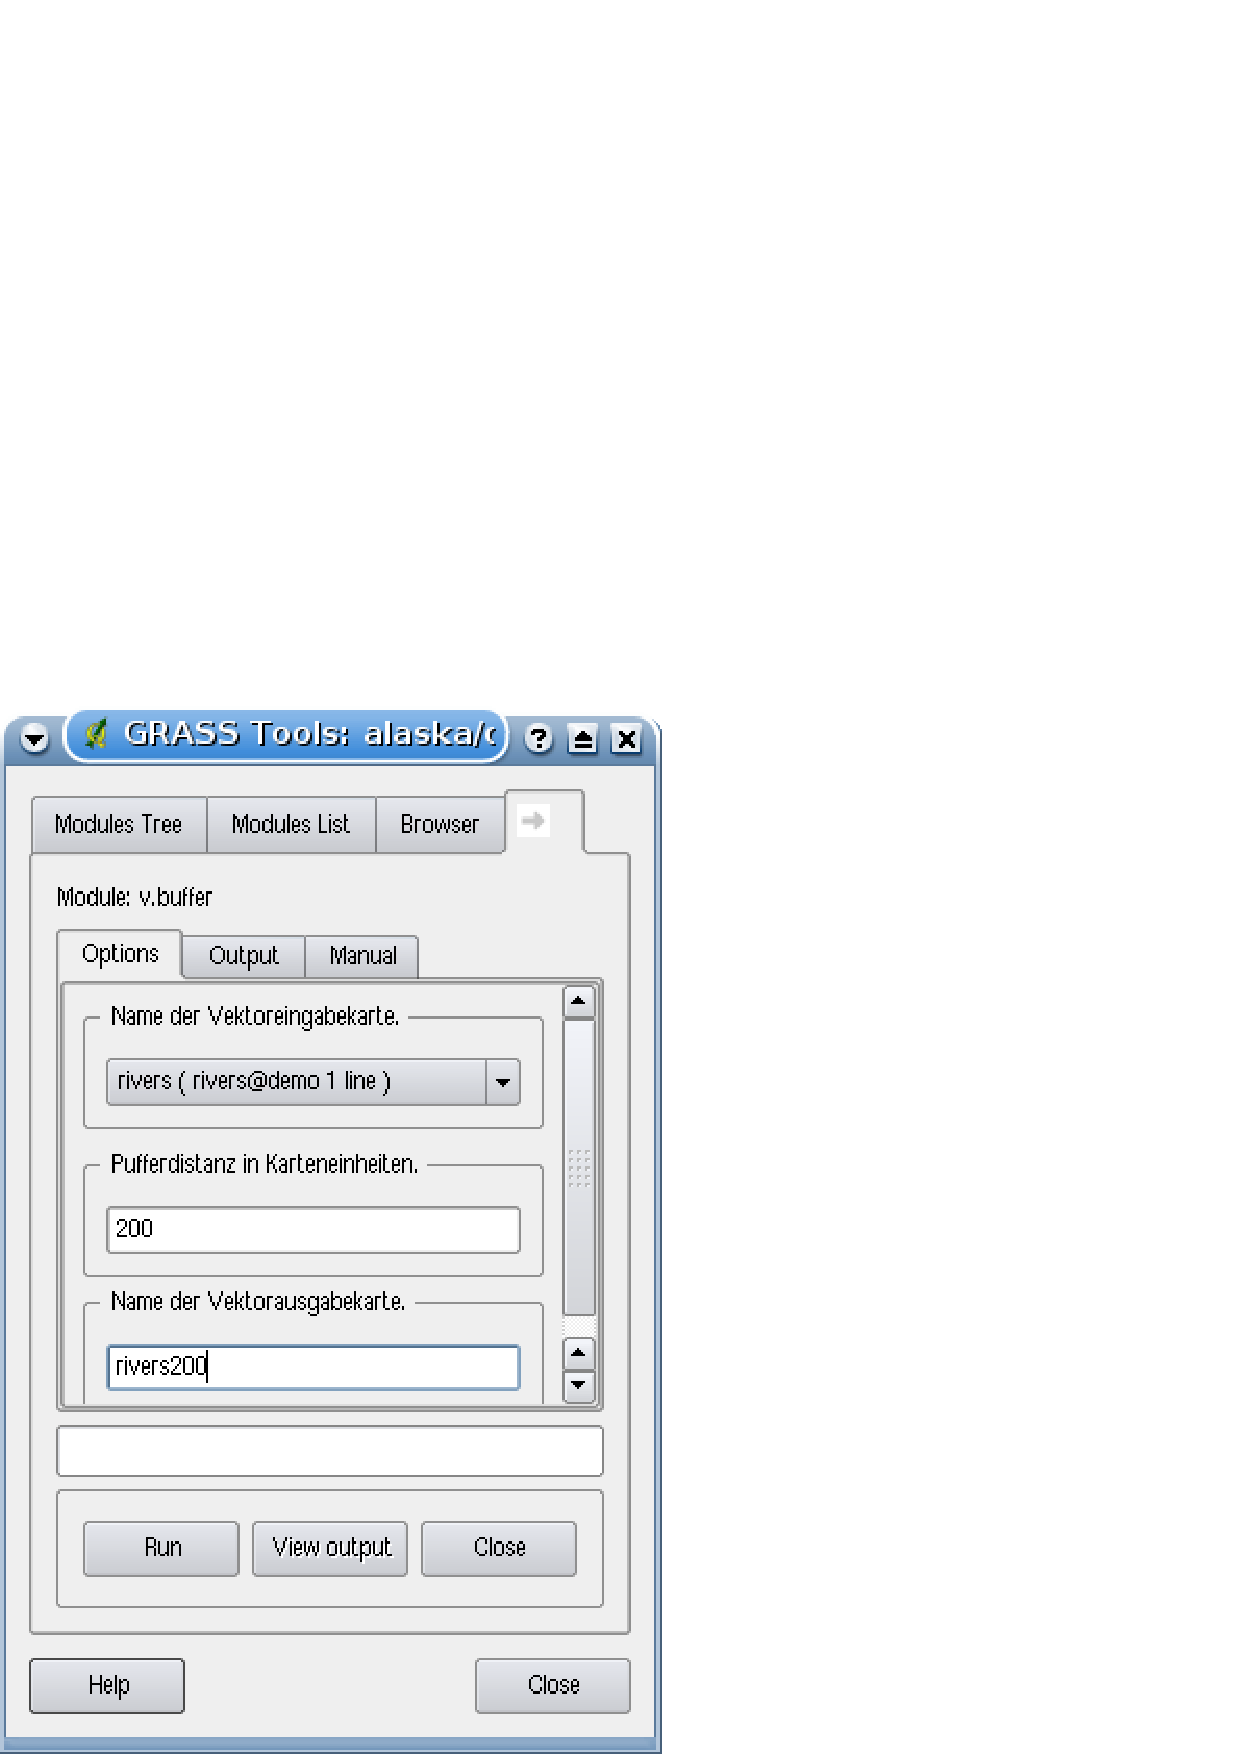
\includegraphics[clip=true, width=0.3\textwidth]{grass_module_option}}\goodgap
   \subfigure[Rendu du module] {\label{subfig:grass_module_output}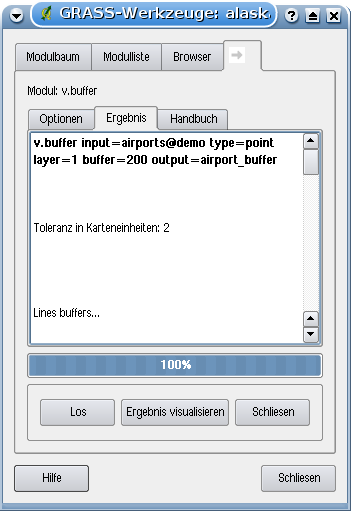
\includegraphics[clip=true, width=0.3\textwidth]{grass_module_output}}\goodgap
   \subfigure[Aide sur le module] {\label{subfig:grass_module_manual}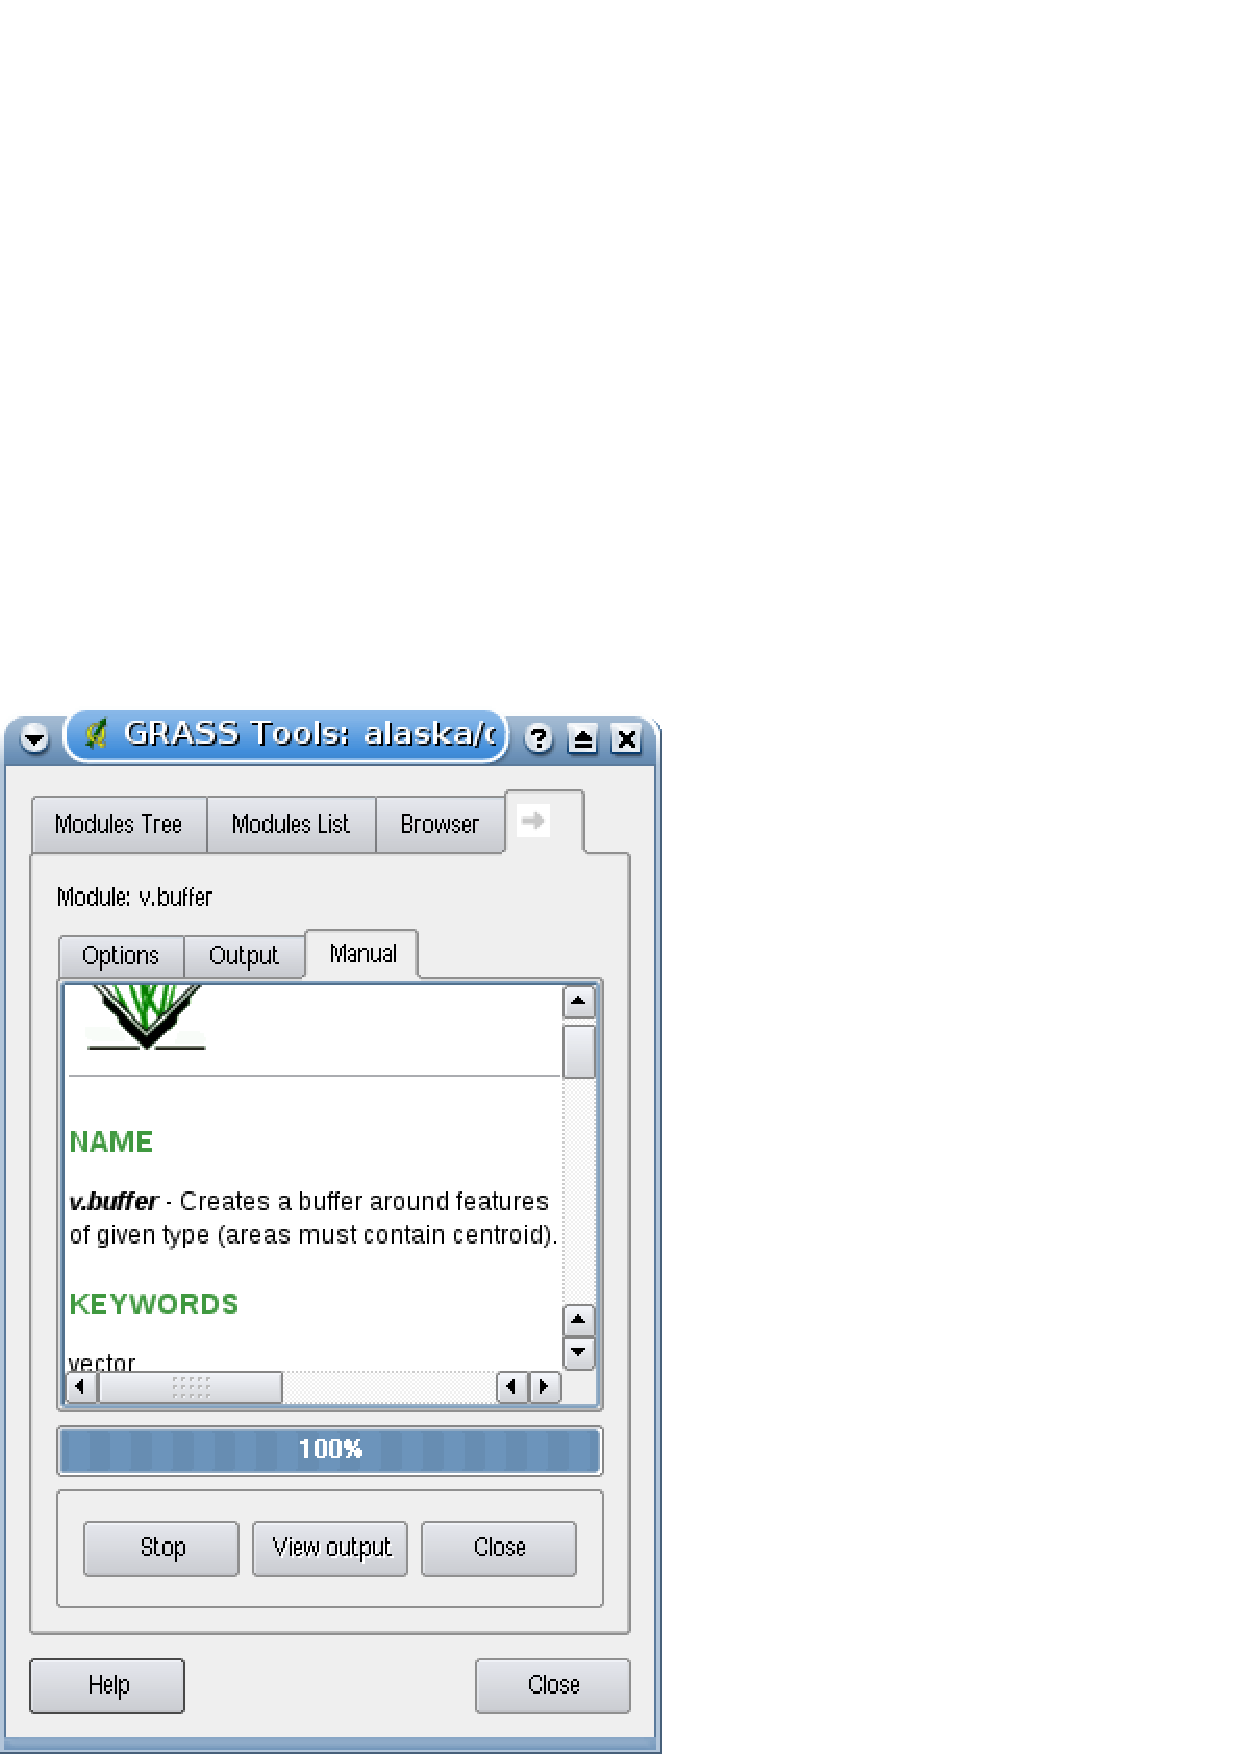
\includegraphics[clip=true, width=0.3\textwidth]{grass_module_manual}}
\end{figure}

\minisec{Options}

%The \tab{Options} tab provides a simplified module dialog where you can usually select a raster or vector layer visualized in the QGIS canvas and 
%enter further module specific parameters to run the module. The provided module parameters are often not complete to keep the dialog clear. If you want to use further module parameters and flags, you need to start the GRASS Shell and run the module in the command line.
L'onglet \tab{Options} propose une interface simplifi\'ee o\`u vous pouvez s\'electionner un raster ou un vecteur en cours de visualisation dans QGIS et
saisir les param\`etres sp\'ecifiques au module avant de le lancer. Tous les param\`etres du module ne sont g\'en\'eralement pas fournis afin de simplifier
les bo\^ites de dialogue. Pour utiliser des param\`etres que ne se trouvent pas dans la bo\^ite de dialogue, vous devez utiliser l'invite de commande
et lancer les modules en lignes de commande.

%\minisec{Output}
\minisec{Rendu}

%The \tab{Output} tab provides information about the output status of the module. When you click the \button{Run} button, the module switches to the 
%\tab{Output} tab and you see information about the analysis process. If all works well, you will finally see a \usertext{Successfully finished} message.
L'onglet \tab{Rendu} fournit des informations sur l'\'etat de sortie du module. Quand vous cliquez sur le bouton \button{Lancer}, le module passe sur l'onglet \tab{Rendu} et vous voyez les informations sur le processus en cours. Si tout se passe bien, vous verrez finalement le message \usertext{Termin\'e avec succ\`es}.
%\minisec{Manual}
\minisec{Manuel}

%The \tab{Manual} tab shows the HTML help page of the GRASS module. You can use it to check further module parameters and flags or to get a deeper 
%knowledge about the purpose of the module. At the end of each module manual page you see further links to the \filename{Main Help index}, the 
%\filename{Thematic index} and the \filename{Full index}. These links provide the same information as if you use the module \filename{g.manual}.
L'onglet \tab{Manuel} montre la page HTML d'aide du module. Vous pouvez vous en servir pour voir les autres param\`etres du modules et pour avoir une
connaissance plus approfondie de l'objet du module. A la fin de chaque page d'aide d'un module, vous avez des liens vers \filename{Main Help index},
\filename{Thematic index} et \filename{Full index}. Ces liens vous donnent les m\^emes informations que si vous utilisiez \filename{g.manual}.

%\begin{Astuce}\caption{\textsc{Display results immediately}}\index{GRASS!display results}
\begin{Astuce}\caption{\textsc{Afficher les r\'esultats imm\'ediatement}}\index{GRASS!afficher les r\'esultats}
%\qgistip{If you want to display your calculation results immediately in your map canvas, you can use the 'View Output' button at the bottom of the  module tab.
\qgistip{Si vous voulez voir imm\'ediatement dans votre fen\^etre carte le r\'esultat du module, vous pouvez utiliser le bouton 'Vue' au bas de l'onglet du module.
}
\end{Astuce} 

%\subsubsection{Working with the GRASS LOCATION browser} \index{GRASS!toolbox!Browser}
\subsubsection{Travailler avec le navigateur GRASS} \index{GRASS!bo\^ite \`a outils!navigateur}

%Another useful feature inside the GRASS Toolbox is the GRASS \filename{LOCATION} browser. In Figure~\ref{fig:grass_mapset_browser} you 
%can see the current working \filename{LOCATION} with its \filename{MAPSETs}.
Une autre fonctionnalit\'e utile dans la bo\^ite \`a outils GRASS est le navigateur de \filename{SECTEUR} GRASS. Sur la figure~\ref{fig:grass_mapset_browser}
vous pouvez voir le \filename{SECTEUR} en cours  avec ses \filename{Jeux de Donn\'ees}. 

%In the left browser windows you can browse through all \filename{MAPSETs} inside the current \filename{LOCATION}. The right browser window shows some  meta information for selected raster or vector layers, e.g. resolution, bounding box, data source, connected attribute table for vector data and a  command history.
Dans la partie gauche de la fen\^etre vous pouvez naviguer dans tous les \filename{Jeux de Donn\'ees} du \filename{SECTEUR} courant. La partie droite de la fen\^etre affiche des informations sur le raster ou le vecteur s\'electionn\'e, tel que la r\'esolution, l'emprise, la source des donn\'ees, les tables attributaires pour les vecteurs et un historique des commandes.


\begin{figure}[h]
 \begin{center}
% \caption{GRASS LOCATION browser \nixcaption}\label{fig:grass_mapset_browser}
 \caption{Navigateur de SECTEUR GRASS \nixcaption}\label{fig:grass_mapset_browser}
 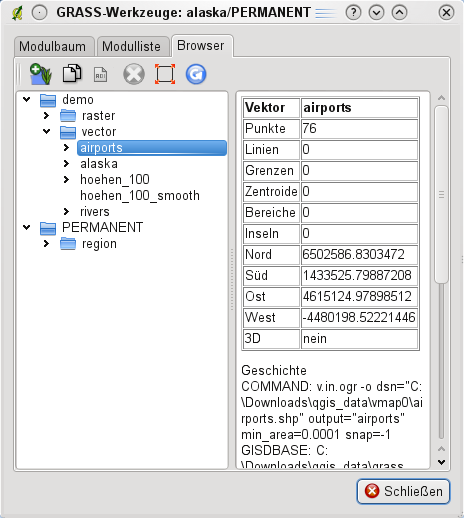
\includegraphics[clip=true,width=10cm]{grass_mapset_browser}
 \end{center}
\end{figure}

%The toolbar inside the \tab{Browser} tab offers following tools to manage the selected \filename{LOCATION}:
La barre d'outils de l'onglet \tab{Parcourir} donne acc\`es \`a des outils de gestion du \filename{SECTEUR} s\'electionn\'e :

\begin{itemize}
%\item \toolboxtwo{grass_add_map}{Add selected map to canvas}
%\item \toolboxtwo{grass_copy_map}{Copy selected map}
%\item \toolboxtwo{grass_rename_map}{Rename selected map}
%\item \toolboxtwo{grass_delete_map}{Delete selected map}
%\item \toolboxtwo{grass_set_region}{Set current region to selected map}
%\item \toolboxtwo{grass_refresh}{Refresh browser window}
\item \toolboxtwo{grass_add_map}{Ajoute la carte s\'electionn\'ee \`a la carte QGIS}
\item \toolboxtwo{grass_copy_map}{Copie la carte s\'electionn\'ee}
\item \toolboxtwo{grass_rename_map}{Renomme la carte s\'electionn\'ee}
\item \toolboxtwo{grass_delete_map}{Efface la carte s\'electionn\'ee}
\item \toolboxtwo{grass_set_region}{R\'egion courante r\'egl\'ee sur la carte choisie}
\item \toolboxtwo{grass_refresh}{Rafra\^ichir}

\end{itemize}

%The \toolboxtwo{grass_rename_map}{Rename selected map} and \toolboxtwo{grass_delete_map}{Delete selected map} only work with maps inside 
%your currently selected \filename{MAPSET}. All other tools also work with raster and vector layers in another \filename{MAPSET}.
Les commandes \toolboxtwo{grass_rename_map}{Renomme la carte s\'electionn\'ee} et \toolboxtwo{grass_delete_map}{Efface la carte s\'electionn\'ee} ne fonctionnent qu'avec les cartes pr\'esente dans votre \filename{Jeu de Donn\'ees} s\'electionn\'e. Tous les autres outils fonctionnent aussi avec les autres \filename{Jeux de Donn\'ees}.

%\subsubsection{Customizing the GRASS Toolbox} \index{GRASS!toolbox!customize}
\subsubsection{Personnaliser la bo\^ite \`a outils GRASS} \index{GRASS!bo\^ite \`a outils!personnaliser}
\label{sec:toolbox-customizing}

%Nearly all GRASS modules can be added to the GRASS toolbox. A XML interface is provided to parse the pretty simple XML files which configures 
%the modules appearance and parameters inside the toolbox.
Pratiquement tous les modules GRASS peuvent \^etre ajout\'es \`a la bo\^ite \`a outils. Une interface XML est fournie pour analyser les fichiers XML 
tr\`es simple qui configurent l'apparence et les param\`etres des modules dans la bo\^ite \`a outils.

%A sample XML file for generating the module \usertext{v.buffer} (v.buffer.qgm) looks like this:
Un exemple de fichier XML pour le module \usertext{v.buffer} (v.buffer.qgm) est donn\'e ci-dessous :
\begin{verbatim}
<?xml version="1.0" encoding="UTF-8"?>
<!DOCTYPE qgisgrassmodule SYSTEM "http://mrcc.com/qgisgrassmodule.dtd">

<qgisgrassmodule label="Vector buffer" module="v.buffer">
        <option key="input" typeoption="type" layeroption="layer" />
        <option key="buffer"/>
        <option key="output" />
</qgisgrassmodule>
\end{verbatim}

%The parser reads this definition and creates a new tab inside the toolbox when you select the module. A more detailed description for adding new  modules, changing the modules group, etc. can be found on the QGIS wiki at \\\url{http://wiki.qgis.org/qgiswiki/Adding\_New\_Tools\_to\_the\_GRASS\_Toolbox}.
L'analyseur lit cette d\'efinition et cr\'ee un nouvel onglet \`a l'int\'erieur de la bo\^ite \`a outils lorsque vous s\'electionnez le module. Une description plus d\'etaill\'ee pour ajouter des modules, changer le groupe des modules, etc. est disponible sur le wiki QGIS \`a l'adresse \\\url{http://wiki.qgis.org/qgiswiki/Adding\_New\_Tools\_to\_the\_GRASS\_Toolbox}.